\documentclass[10pt,fleqn]{wlpeerj}
\usepackage{lineno}
\usepackage{unicode-math}
\setmainfont
[    Extension = .otf,
   UprightFont = *-regular,
      BoldFont = *-bold,
    ItalicFont = *-italic,
BoldItalicFont = *-bolditalic,
]{xits}
\setmathfont
[    Extension = .otf,
      BoldFont = *bold,
]{xits-math}
\linenumbers
\usepackage{ifxetex,ifluatex}
\usepackage[CJK]{ucharclasses} %provides fontreplacement
\usepackage{fixltx2e} % provides \textsubscript
\ifnum 0\ifxetex 1\fi\ifluatex 1\fi=0 % if pdftex
  \usepackage[T1]{fontenc}
  \usepackage[utf8]{inputenc}
%\else % if luatex or xelatex
%  \ifxetex
%    \usepackage{mathspec}
%  \else
%    \usepackage{fontspec}
%  \fi
\defaultfontfeatures{Ligatures=TeX,Scale=MatchLowercase}
\fi
% use upquote if available, for straight quotes in verbatim environments
\IfFileExists{upquote.sty}{\usepackage{upquote}}{}
\usepackage[unicode=true]{hyperref}
\usepackage{longtable,booktabs}
% Fix footnotes in tables (requires footnote package)
\IfFileExists{footnote.sty}{\usepackage{footnote}\makesavenoteenv{long table}}{}
\usepackage{graphicx,grffile}
\makeatletter
\def\maxwidth{\ifdim\Gin@nat@width>\linewidth\linewidth\else\Gin@nat@width\fi}
\def\maxheight{\ifdim\Gin@nat@height>\textheight\textheight\else\Gin@nat@height\fi}
\makeatother
% Scale images if necessary, so that they will not overflow the page
% margins by default, and it is still possible to overwrite the defaults
% using explicit options in \includegraphics[width, height, ...]{}
\setkeys{Gin}{width=\maxwidth,height=\maxheight,keepaspectratio}
\IfFileExists{parskip.sty}{%
\usepackage{parskip}
}{% else
\setlength{\parindent}{0pt}
\setlength{\parskip}{6pt plus 2pt minus 1pt}
}
\setlength{\emergencystretch}{3em}  % prevent overfull lines
\providecommand{\tightlist}{%
  \setlength{\itemsep}{0pt}\setlength{\parskip}{0pt}}
\setcounter{secnumdepth}{0}
% Redefines (sub)paragraphs to behave more like sections
\ifx\paragraph\undefined\else
\let\oldparagraph\paragraph
\renewcommand{\paragraph}[1]{\oldparagraph{#1}\mbox{}}
\fi
\ifx\subparagraph\undefined\else
\let\oldsubparagraph\subparagraph
\renewcommand{\subparagraph}[1]{\oldsubparagraph{#1}\mbox{}}
\fi


% set default figure placement to htbp
\makeatletter
\def\fps@figure{htbp}
\makeatother


\title{Formatting
Open
Science:
agile
creation
of
multiple
document
types
by
writing
academic
manuscripts
in
pandoc
markdown}

\author{Albert
Krewinkel\(^1\)
and
Robert
Winkler\(^{2,\star}\)}



\date{}

\begin{document}

\flushbottom
\maketitle
\thispagestyle{empty}

\textbf{Affiliations:}
¹ TBD
(Pandoc
Development
Team),
²
CINVESTAV
Unidad
Irapuato,
Department
of
Biochemistry
and
Biotechnology,
Laboratory
of
Biochemical
and
Instrumental
Analysis,
Km.
9.6
Libramiento
Norte
Carr.
Irapuato-León,
36821
Irapuato,
Gto.
Mexico

\textbf{Correspondence:}
Prof.~Dr.~Robert
Winkler,
\href{mailto:robert.winkler@cinvestav.mx}{\nolinkurl{robert.winkler@cinvestav.mx}}

\textbf{Keywords:}
open
science,
document
formats,
markdown,
latex,
publishing,
typesetting

\section{Abstract}\label{abstract}

The
timely
publication
of
scientific
results
is
essential
for
dynamic
advances
in
science.
The
ubiquitous
availability
of
computers
which
are
connected
to a
global
network
made
the
rapid
and
low-cost
distribution
of
information
through
electronic
channels
possible.
New
concepts,
such
as
Open
Access
publishing
and
preprint
servers
are
currently
changing
the
traditional
print
media
business
towards
a
community-driven
peer
production.
However,
the
cost
of
scientific
literature
generation,
which
is
either
charged
to
readers,
authors
or
sponsors,
is
still
high.
The
main
active
participants
in
the
authoring
and
evaluation
of
scientific
manuscripts
are
volunteers,
and
the
cost
for
online
publishing
infrastructure
is
close
to
negligible.
A
major
time
and
cost
factor
though
is
the
formatting
of
manuscripts
in
the
production
stage.
In
this
article
we
demonstrate
the
feasibility
to
write
scientific
manuscripts
in
plain
markdown
(MD)
text
files,
which
can
be
easily
converted
into
common
publication
formats,
such
as
PDF,
HTML
or
EPUB,
using
pandoc.
The
simple
syntax
of
markdown
assures
the
long-term
readability
of
raw
files
and
the
development
of
software
and
workflows.
We
show
the
implementation
of
typical
elements
of
scientific
manuscripts
--
formulas,
tables,
code
blocks
and
citations
--
and
present
tools
for
editing,
collaborative
writing
and
version
control.
We
give
an
example
on
how
to
prepare
a
manuscript
with
distinct
output
formats,
a
DOCX
file
for
submission
to a
journal
and a
LATEX/PDF
version
for
deposition
as a
PeerJ
preprint.
Reducing
the
work
spent
on
manuscript
formatting
translates
directly
to
time
and
cost
savings
for
writers,
publishers,
readers
and
sponsors.
Therefore,
the
adoption
of
the
MD
format
contributes
to
the
agile
production
of
open
science
literature.

\section{Introduction}\label{introduction}

Agile
development
of
science
depends
on
the
continuous
exchange
of
information
between
the
researchers
\citep{woelfle_open_2011}.
In
the
past,
physical
copies
of
scientific
works
had
to be
produced
and
distributed.
Therefore,
publishers
needed
to
invest
considerable
economical
resources
for
typesetting
and
printing.
Since
the
journals
were
mainly
financed
by
their
subscribers,
their
editors
not
only
had
to
decide
on
the
scientific
quality
of a
submitted
manuscript,
but
also
on
the
potential
interest
for
their
readers.
The
availability
of
globally
connected
computers
enabled
the
rapid
exchange
of
information
at
low
cost.
Yochai
Benkler
(2006)
predicts
important
changes
in
the
information
production
economy,
which
are
based
on
three
observations:

\begin{enumerate}
\def\labelenumi{\arabic{enumi}.}
\tightlist
\item
  A
  nonmarket
  motivation
  in
  areas
  such
  as
  education,
  arts,
  science,
  politics
  and
  theology.
\item
  The
  actual
  rise
  of
  nonmarket
  production,
  made
  possible
  through
  networked
  individuals
  and
  coordinate
  effects.
\item
  The
  emergence
  of
  large-scale
  peer
  production,
  e.g.~of
  software
  and
  encyclopaedias.
\end{enumerate}

Immaterial
goods
such
as
knowledge
and
culture
are
not
lost,
when
consumed
or
shared
--
they
are
`nonrival'
--,
and
they
enable
a
networked
information
economy,
which
is
not
commercially
driven
\citep{benkler_wealth_2006}.

\subsection{Preprints
and
e-prints}\label{preprints-and-e-prints}

In
some
areas
of
science
already
existed
a
preprint
culture,
i.e.~a
paper-based
exchange
system
of
research
ideas
and
results,
when
Paul
Ginsparg
in
1991
initiated
a
server
for
the
distribution
of
electronic
preprints
--
`e-prints'
--
about
high-energy
particle
theory
at
the
Los
Alamos
National
Laboratory
(LANL),
USA
\citep{ginsparg_first_1994}.
Later,
the
LANL
server
moved
with
Ginsparg
to
Cornell
University,
USA,
and
was
renamed
to
arXiv
\citep{butler_alamos_2001}.
Currently,
arXiv
(\url{https://arxiv.org/})
publishes
e-prints
related
to
physics,
mathematics,
computer
science,
quantitative
biology
quantitative
finance
and
statistics.
Just
a few
years
after
the
start
of
the
first
preprint
servers,
their
important
contribution
to
scientific
communication
was
evident
\citep{ginsparg_first_1994, youngen_citation_1998, brown_e-volution_2001}.
In
2014,
arXiv
reached
the
impressive
number
of 1
million
e-prints
\citep{van_noorden_arxiv_2014}.
In
more
conservative
areas,
such
as
chemistry
and
biology,
accepting
the
publishing
prior
peer-review
took
more
time
\citep{brown_role_2003}.
A
preprint
server
for
life
sciences
(\url{http://biorxiv.org/})
was
launched
by
the
Cold
Spring
Habor
Laboratory,
USA,
in
2013
\citep{callaway_preprints_2013}.
\emph{PeerJ
preprints}
(\url{https://peerj.com/preprints/}),
started
in
the
same
year,
accepts
manuscripts
from
biological
sciences,
medical
sciences,
health
sciences
and
computer
sciences.
The
terms
`preprints'
and
`e-prints'
are
used
synonymously,
since
the
physical
distribution
of
preprints
has
become
obsolete.
A
major
drawback
of
preprint
publishing
are
the
sometimes
restrictive
policies
of
scientific
publishers.
The
SHERPA/RoMEO
project
informs
about
copyright
policies
and
self-archiving
options
of
individual
publishers
(\url{http://www.sherpa.ac.uk/romeo/}).

\subsection{Open
Access}\label{open-access}

The
term
\emph{`Open
Access'}
was
introduced
2002
by
the
Budapest
Open
Access
Initiative
and
was
defined
as:

\emph{``Barrier-free
access
to
online
works
and
other
resources.
OA
literature
is
digital,
online,
free
of
charge
(gratis
OA),
and
free
of
needless
copyright
and
licensing
restrictions
(libre
OA).''}
\citep{suber_open_2012}

Frustrated
by
the
difficulty
to
access
even
digitalized
scientific
literature,
three
scientists
founded
the
\emph{Public
Library
of
Science
(PLoS)}.
In
2003,
\emph{PLoS
Biology}
was
published
as
the
first
fully
Open
Access
(OA)
journal
for
biology
\citep{brown_why_2003, eisen_publish_2003}.
Thanks
to
the
great
success
of OA
publishing,
many
conventional
print
publishers
now
offer
a
so-called
`Open
Access
option',
i.e.~to
make
accepted
articles
free
to
read
for
an
additional
payment.
The
copyright
in
this
hybrid
models
might
remain
with
the
publisher,
whilst
fully
OA
usually
provide
a
liberal
license,
such
as
the
Creative
Commons
Attribution
4.0
International
(CC
BY
4.0,
\url{https://creativecommons.org/licenses/by/4.0/}).
OA
literature
is
only
one
component
of a
more
general
\emph{open}
philosophy,
which
also
includes
the
access
to
scholarships,
software,
and
data
\citep{willinsky_unacknowledged_2005}.
Interestingly,
there
are
several
different
`schools'
of
thinking
on
how
to
understand
and
define
\emph{Open
Science},
as
well
the
position
that
any
science
is
open
by
definition,
because
of
its
objective
to
make
generated
knowledge
public
\citep{fecher_open_2014}.

\subsection{Cost
of
journal
article
production}\label{cost-of-journal-article-production}

In a
recent
study,
the
article
processing
charges
(APCs)
for
research
intensive
universities
in
the
USA
and
Canada
were
estimated
to be
about
1,800
USD
for
fully
OA
journals
and
3,000
USD
for
hybrid
OA
journals
\citep{solomon_article_2016}.
PeerJ
(\url{https://peerj.com/}),
an OA
journal
for
biological
and
computer
sciences
launched
2013,
drastically
reduced
the
publishing
cost
and
offers
its
members
a
life-time
publishing
plan
for a
small
registration
fee
\citep{van_noorden_journal_2012};
alternatively
the
authors
can
choose
to
pay
an
APC
of
1,095
USD,
which
may
be
cheaper,
if
multiple
co-authors
participate.
Examples
such
as
the
\emph{Journal
of
Statistical
Software}
(\emph{JSS},
\url{https://www.jstatsoft.org/})
and
\emph{eLife}
(\url{https://elifesciences.org/})
demonstrate
the
possibility
of
completely
community-supported
OA
publications.
\textbf{Fig.
1}
compares
the
APCs
of
different
OA
publishing
business
models.
\emph{JSS}
and
\emph{eLife}
are
peer-reviewed
and
indexed
by
Thomson
Reuters.
Both
journals
are
located
in
the
Q1
quality
quartile
in
all
their
registered
subject
categories
of
the
Scimago
Journal
\&
Country
Rank
(\url{http://www.scimagojr.com/}),
demonstrating
that
high-quality
publications
can
be
produced
without
charging
the
scientific
authors
or
readers.

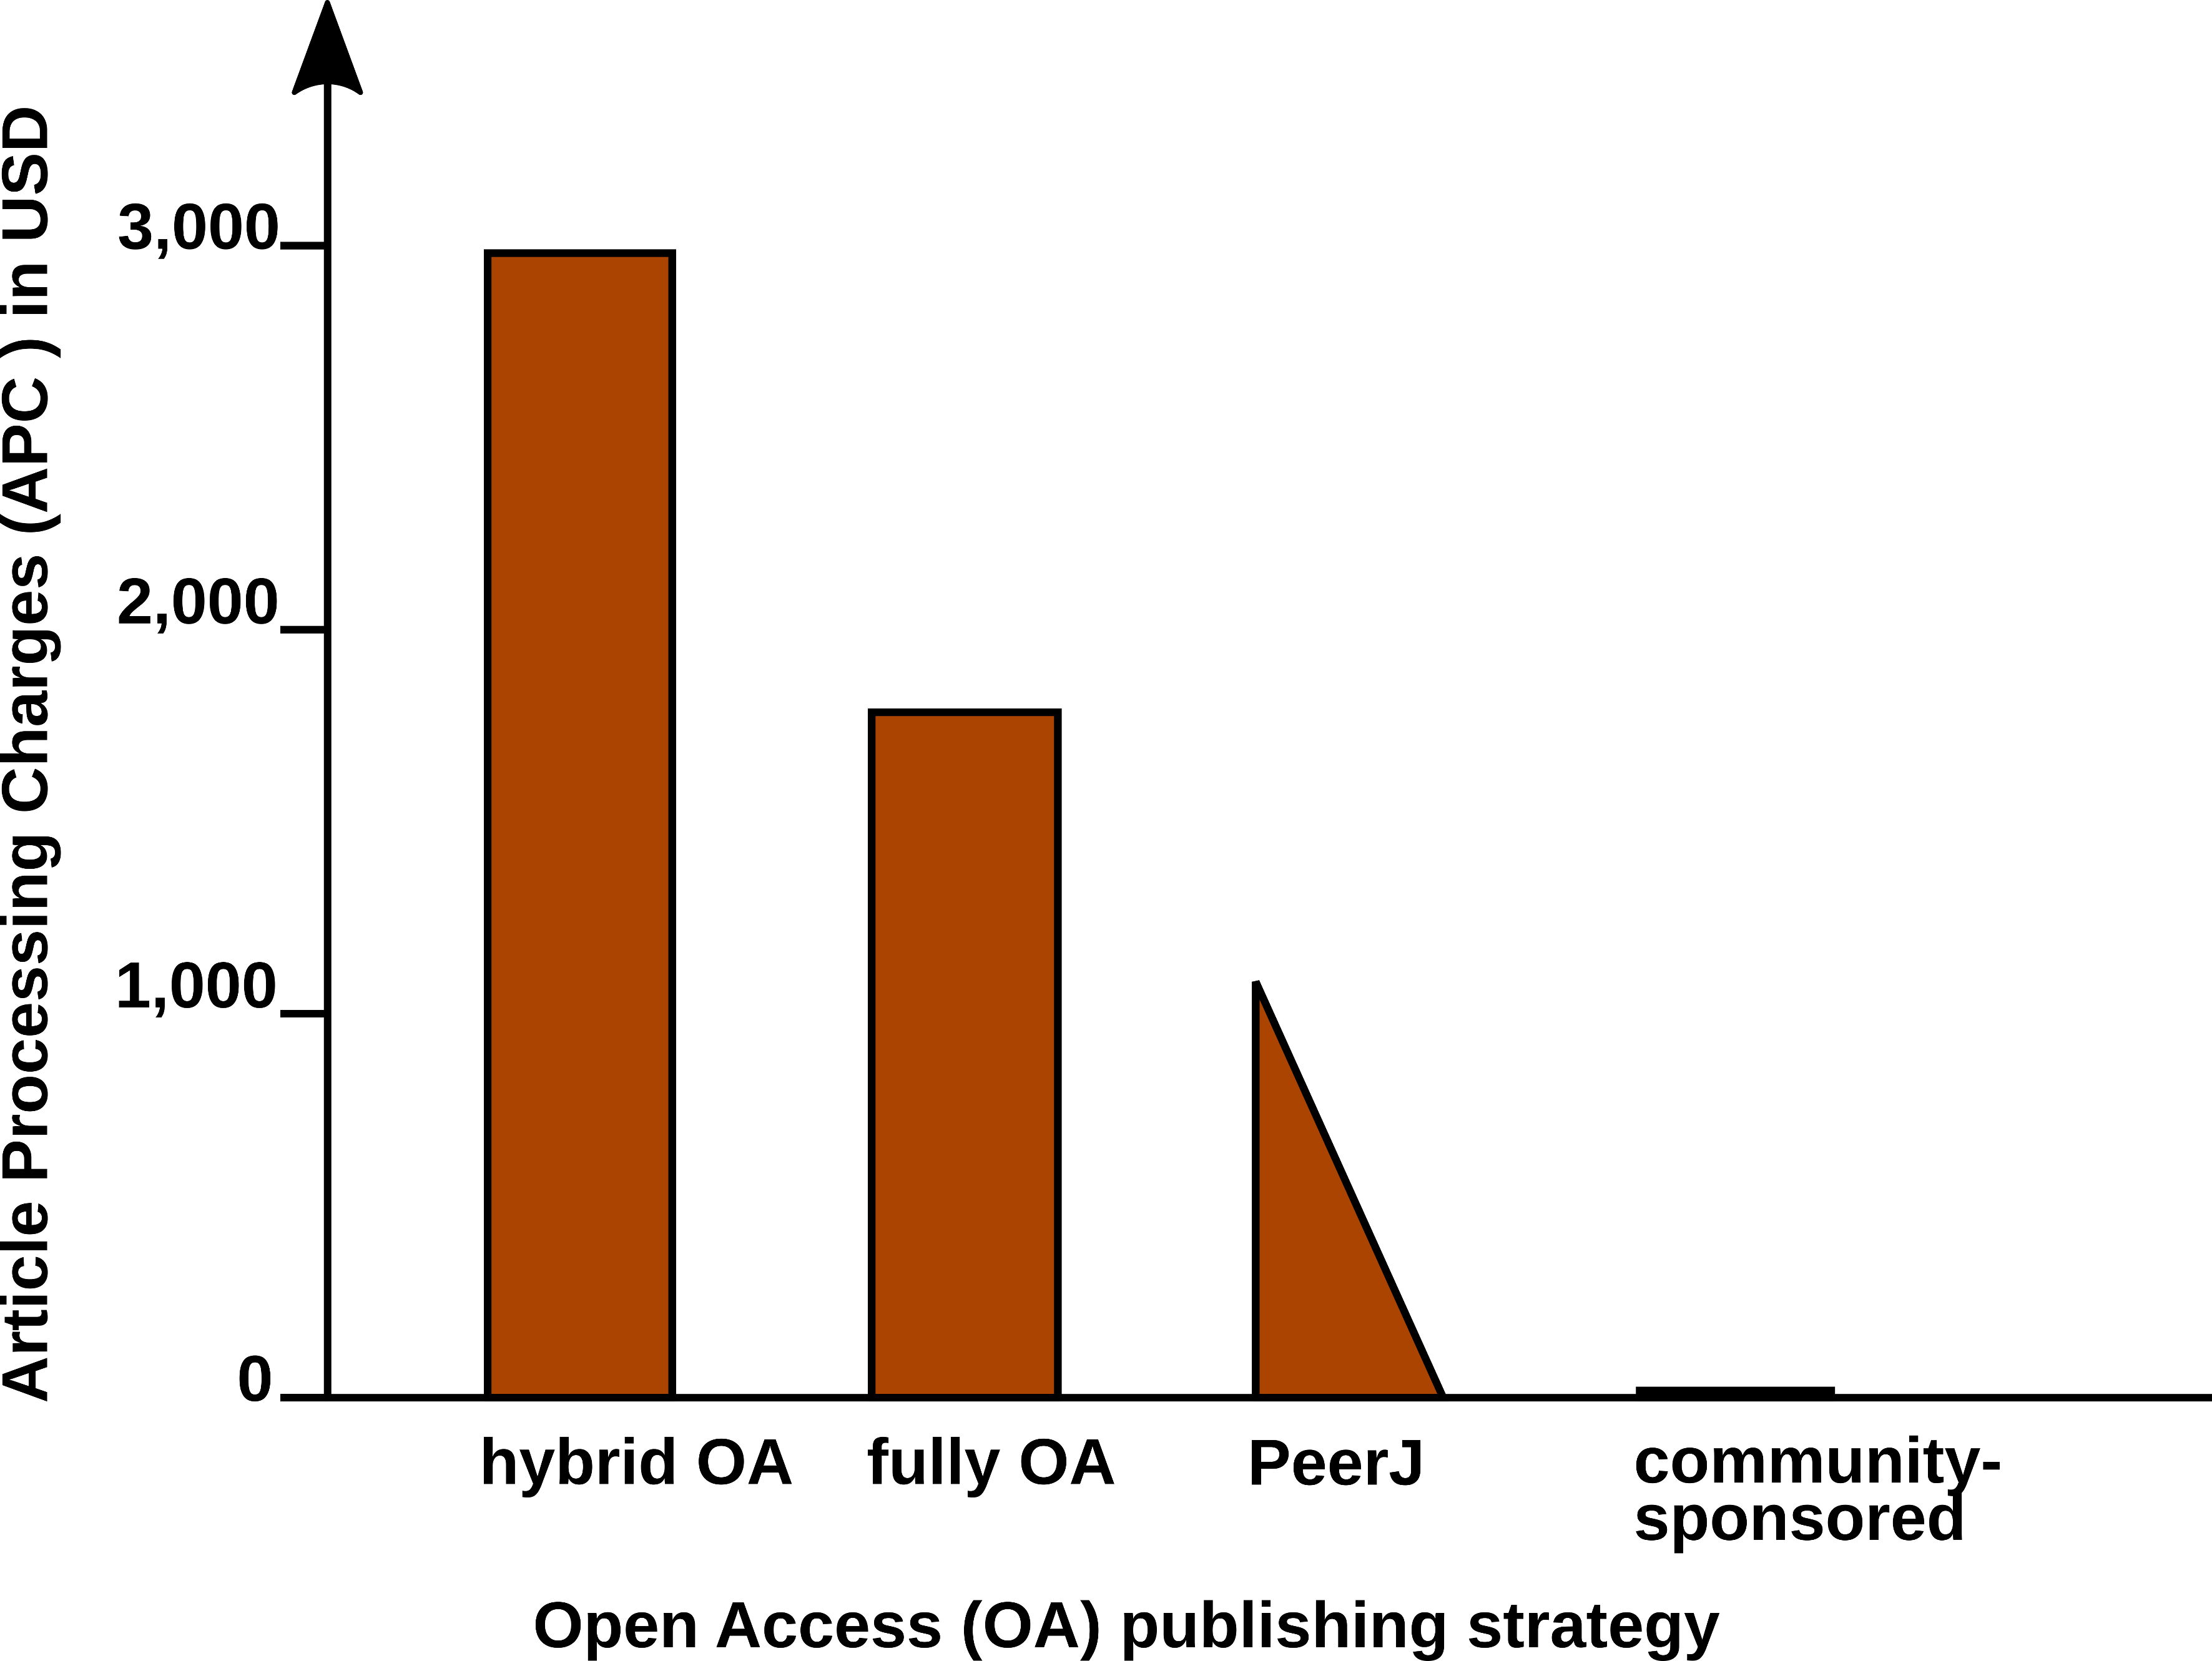
\includegraphics{fig-OA-strategies-APCs.png}
\textbf{Figure
1.}
Article
Processing
Charge
(APCs)
that
authors
have
to
pay
for
with
different
Open
Access
(OA)
publishing
models.
Data
from
\citep{solomon_article_2016}
and
journal
webpages.

In
2009,
a
study
was
carried
concerning
the
\emph{``Economic
Implications
of
Alternative
Scholarly
Publishing
Models''},
which
demonstrates
an
overall
societal
benefit
by
using
OA
publishing
model
\citep{houghton_economic_2009}.
In
the
same
report,
the
real
publication
costs
are
evaluated.
The
relative
costs
of an
article
for
the
publisher
are
represented
in
\textbf{Fig.
2}.

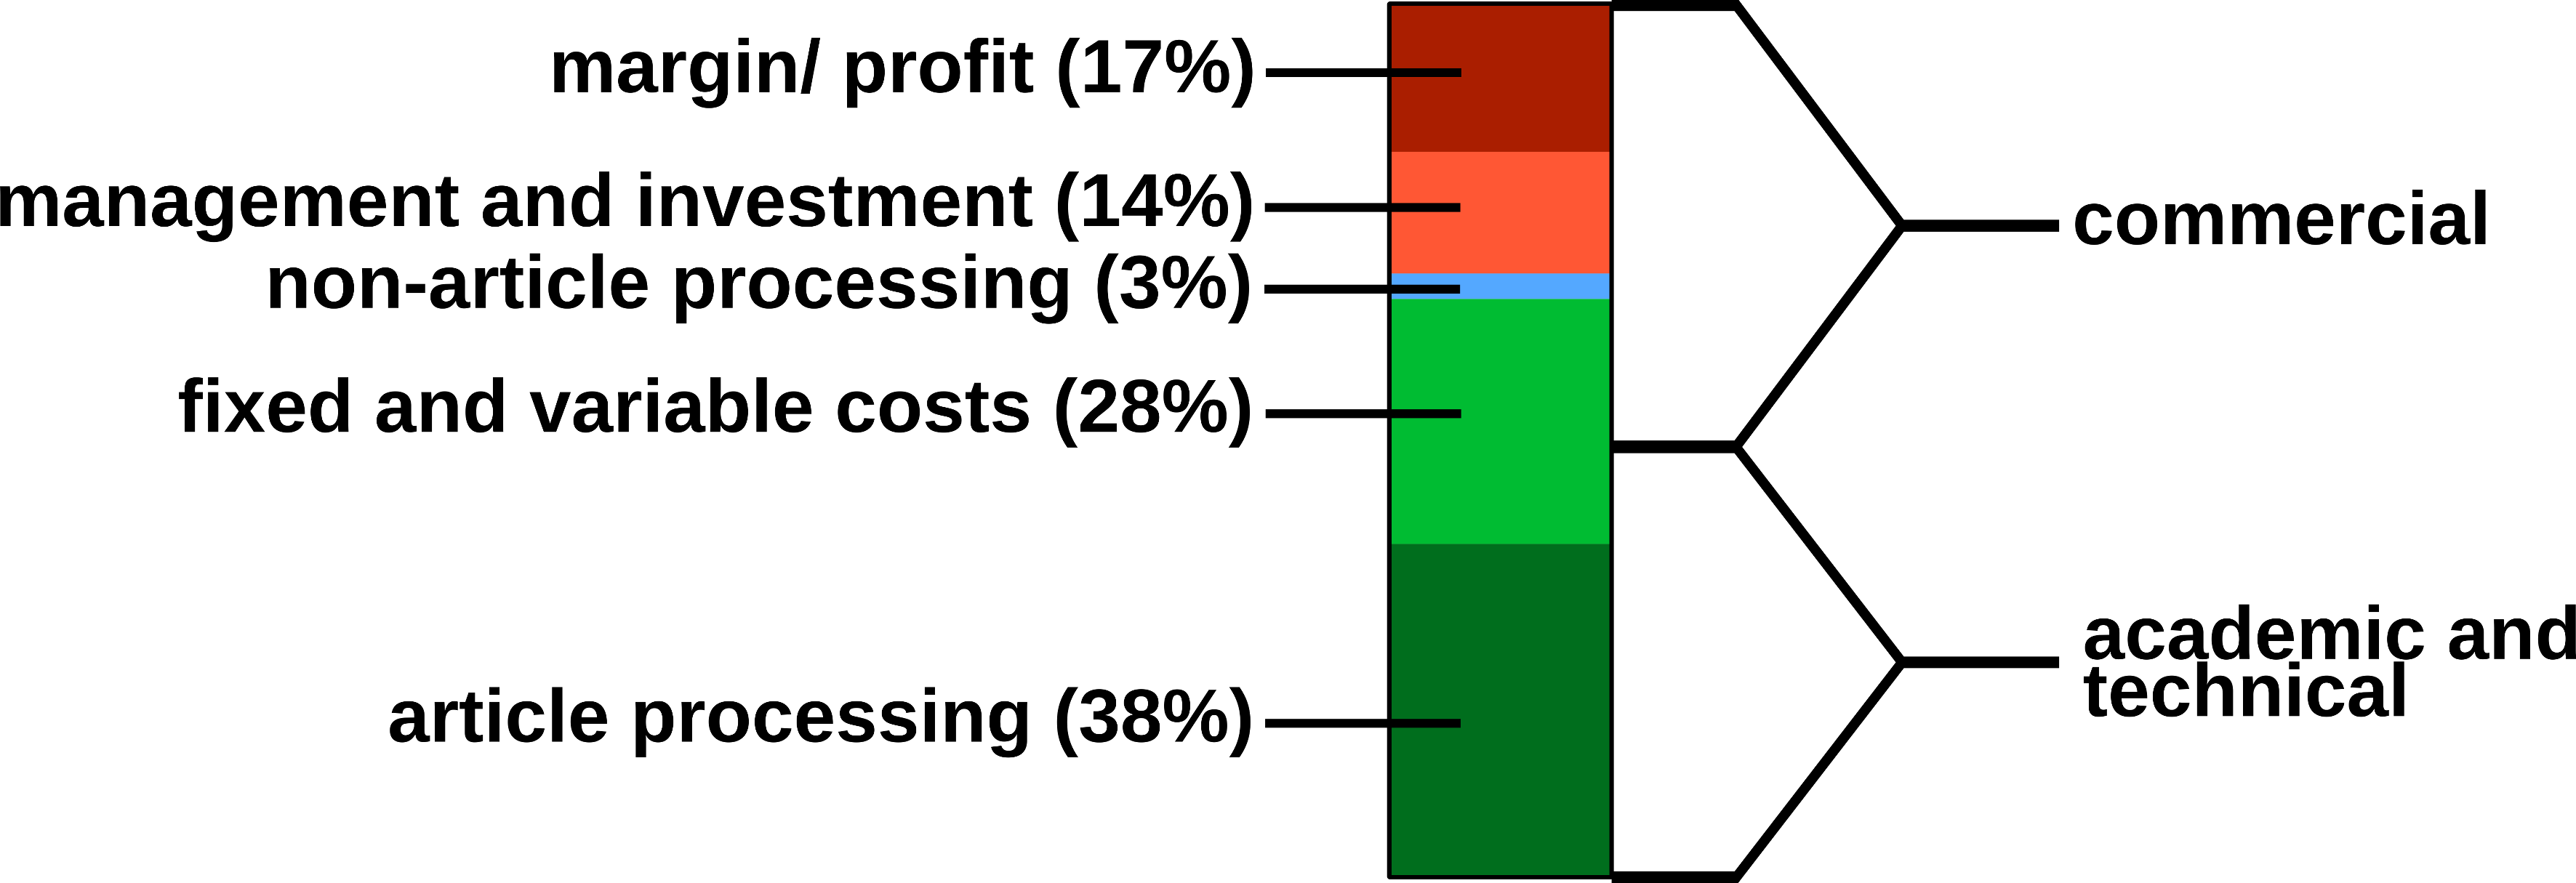
\includegraphics{fig-hybrid-publishing-costs.png}
\textbf{Figure
2.}
Estimated
publishing
cost
for a
`hybrid'
journal
(conventional
with
Open
Access
option).
Data
from
\citep{houghton_economic_2009}.

Conventional
publishers
justify
their
high
subscription
or
APC
prices
with
the
added
value,
e.g.~journalism
(stated
in
the
graphics
as
`non-article
processing').
But
also
stakeholder
profits,
which
could
be as
high
as
50\%,
must
be
considered,
and
are
withdraw
from
the
science
budget
\citep{van_noorden_open_2013}.
Generally,
the
production
costs
of an
article
could
be
roughly
divided
into
commercial
and
academic/
technical
costs
(\textbf{Fig.
2}).
For
nonmarket
production,
the
commercial
costs
such
as
margins/
profits,
management
etc.
can
be
drastically
reduced.
Hardware
and
services
for
hosting
an
editorial
system,
such
as
Open
Journal
Systems
of
the
Public
Knowledge
Project
(\url{https://pkp.sfu.ca/ojs/})
can
be
provided
by
public
institutions.
Employed
scholars
can
perform
editor
and
reviewer
activities
without
additional
cost
for
the
journals.
Nevertheless,
`article
processing',
which
includes
the
manuscript
handling
during
peer
review
and
production
represents
the
most
expensive
part.
Therefore,
we
investigated
a
strategy
for
the
efficient
formatting
of
scientific
manuscripts.

\subsection{Current
standard
publishing
formats}\label{current-standard-publishing-formats}

Generally
speaking,
a
scientific
manuscript
is
composed
from
contents
and
formatting.
Whilst
the
content,
i.e.~text,
figures,
tables,
citations
etc.,
may
remain
the
same
between
different
publishing
forms
and
journal
styles,
the
formatting
can
be
very
different.
Most
publishers
require
the
formatting
of
submitted
manuscripts
in a
certain
format.
Ignoring
this
\textbf{Guide
for
Authors},
e.g.~by
submitting
a
manuscript
with
a
different
reference
style,
gives
a
negative
impression
with
a
journal's
editorial
staff.
Too
carelessly
prepared
manuscripts
can
even
provoke
a
straight
`desk-reject'
\citep{volmer_how_2016}.
Currently
DOC(X),
LATEX
and/
or
PDF
file
formats
are
the
most
frequently
used
for
journal
submission
platforms.
But
even
if
the
content
of a
submitted
manuscript
might
be
accepted
during
the
peer
review
`as
is'
(very
rare),
the
format
still
needs
to be
adjusted
to
the
particular
publication
style
in
the
production
stage.
For
the
electronic
distribution
of
scientific
works,
which
is
gaining
more
and
more
importance,
additional
formats
(EPUB,
(X)HTML)
need
to be
generated.
\textbf{Tab.
1}
lists
the
file
formats
which
are
currently
most
relevant
for
scientific
publishing.

\textbf{Table
1.}
Current
standard
formats
for
scientific
publishing.

\begin{longtable}[]{@{}lllll@{}}
\toprule
\begin{minipage}[b]{0.06\columnwidth}\raggedright\strut
\textbf{Type}
\strut\end{minipage}
&
\begin{minipage}[b]{0.15\columnwidth}\raggedright\strut
\textbf{Description}
\strut\end{minipage}
&
\begin{minipage}[b]{0.13\columnwidth}\raggedright\strut
\textbf{Use}
\strut\end{minipage}
&
\begin{minipage}[b]{0.10\columnwidth}\raggedright\strut
\textbf{Syntax}
\strut\end{minipage}
&
\begin{minipage}[b]{0.41\columnwidth}\raggedright\strut
\textbf{Reference}
\strut\end{minipage}\tabularnewline
\midrule
\endhead
\begin{minipage}[t]{0.06\columnwidth}\raggedright\strut
DOCX
\strut\end{minipage}
&
\begin{minipage}[t]{0.15\columnwidth}\raggedright\strut
Office
Open
XML
\strut\end{minipage}
&
\begin{minipage}[t]{0.13\columnwidth}\raggedright\strut
WYSIWYG
editing
\strut\end{minipage}
&
\begin{minipage}[t]{0.10\columnwidth}\raggedright\strut
XML,
ZIP
\strut\end{minipage}
&
\begin{minipage}[t]{0.41\columnwidth}\raggedright\strut
\citep{OOXML}
\strut\end{minipage}\tabularnewline
\begin{minipage}[t]{0.06\columnwidth}\raggedright\strut
ODT
\strut\end{minipage}
&
\begin{minipage}[t]{0.15\columnwidth}\raggedright\strut
OpenDocument
\strut\end{minipage}
&
\begin{minipage}[t]{0.13\columnwidth}\raggedright\strut
WYSIWYG
editing
\strut\end{minipage}
&
\begin{minipage}[t]{0.10\columnwidth}\raggedright\strut
XML,
ZIP
\strut\end{minipage}
&
\begin{minipage}[t]{0.41\columnwidth}\raggedright\strut
\citep{ODF}
\strut\end{minipage}\tabularnewline
\begin{minipage}[t]{0.06\columnwidth}\raggedright\strut
PDF
\strut\end{minipage}
&
\begin{minipage}[t]{0.15\columnwidth}\raggedright\strut
portable
document
\strut\end{minipage}
&
\begin{minipage}[t]{0.13\columnwidth}\raggedright\strut
print
replacement
\strut\end{minipage}
&
\begin{minipage}[t]{0.10\columnwidth}\raggedright\strut
PDF
\strut\end{minipage}
&
\begin{minipage}[t]{0.41\columnwidth}\raggedright\strut
\citep{international_organization_for_standardization_iso_2013}
\strut\end{minipage}\tabularnewline
\begin{minipage}[t]{0.06\columnwidth}\raggedright\strut
EPUB
\strut\end{minipage}
&
\begin{minipage}[t]{0.15\columnwidth}\raggedright\strut
electronic
publishing
\strut\end{minipage}
&
\begin{minipage}[t]{0.13\columnwidth}\raggedright\strut
ebooks
\strut\end{minipage}
&
\begin{minipage}[t]{0.10\columnwidth}\raggedright\strut
HTML5,
ZIP
\strut\end{minipage}
&
\begin{minipage}[t]{0.41\columnwidth}\raggedright\strut
\citep{eikebrokk_epub_2014}
\strut\end{minipage}\tabularnewline
\begin{minipage}[t]{0.06\columnwidth}\raggedright\strut
LATEX
\strut\end{minipage}
&
\begin{minipage}[t]{0.15\columnwidth}\raggedright\strut
typesetting
system
\strut\end{minipage}
&
\begin{minipage}[t]{0.13\columnwidth}\raggedright\strut
high-quality
print
\strut\end{minipage}
&
\begin{minipage}[t]{0.10\columnwidth}\raggedright\strut
TEX
\strut\end{minipage}
&
\begin{minipage}[t]{0.41\columnwidth}\raggedright\strut
\citep{lamport_latex:_1994}
\strut\end{minipage}\tabularnewline
\begin{minipage}[t]{0.06\columnwidth}\raggedright\strut
HTML
\strut\end{minipage}
&
\begin{minipage}[t]{0.15\columnwidth}\raggedright\strut
hypertext
markup
\strut\end{minipage}
&
\begin{minipage}[t]{0.13\columnwidth}\raggedright\strut
websites
\strut\end{minipage}
&
\begin{minipage}[t]{0.10\columnwidth}\raggedright\strut
(X)HTML
\strut\end{minipage}
&
\begin{minipage}[t]{0.41\columnwidth}\raggedright\strut
\citep{HTML4, HTML5}
\strut\end{minipage}\tabularnewline
\begin{minipage}[t]{0.06\columnwidth}\raggedright\strut
MD
\strut\end{minipage}
&
\begin{minipage}[t]{0.15\columnwidth}\raggedright\strut
Markdown
\strut\end{minipage}
&
\begin{minipage}[t]{0.13\columnwidth}\raggedright\strut
lightweight
markup
\strut\end{minipage}
&
\begin{minipage}[t]{0.10\columnwidth}\raggedright\strut
plain
text
MD
\strut\end{minipage}
&
\begin{minipage}[t]{0.41\columnwidth}\raggedright\strut
\citep{ovadia_markdown_2014, rfc7764}
\strut\end{minipage}\tabularnewline
\bottomrule
\end{longtable}

Although
be
content
elements
of
the
documents
such
as
title,
author,
abstract,
text,
figures,
tables,
etc.
remain
the
same,
the
syntax
of
the
file
formats
is
rather
different.
\textbf{Tab.
2}
demonstrates
some
simple
examples
of
differeces
in
different
markup
languages.

\textbf{Table
2.}
Examples
for
formatting
elements
and
their
implementations
in
different
markup
languages
types.

\begin{longtable}[]{@{}llll@{}}
\toprule
\begin{minipage}[b]{0.20\columnwidth}\raggedright\strut
\textbf{Element}
\strut\end{minipage}
&
\begin{minipage}[b]{0.17\columnwidth}\raggedright\strut
\textbf{Markdown}
\strut\end{minipage}
&
\begin{minipage}[b]{0.25\columnwidth}\raggedright\strut
\textbf{LATEX}
\strut\end{minipage}
&
\begin{minipage}[b]{0.27\columnwidth}\raggedright\strut
\textbf{HTML}
\strut\end{minipage}\tabularnewline
\midrule
\endhead
\begin{minipage}[t]{0.20\columnwidth}\raggedright\strut
\textbf{structure}
\strut\end{minipage}
&
\begin{minipage}[t]{0.17\columnwidth}\raggedright\strut
\strut\end{minipage}
&
\begin{minipage}[t]{0.25\columnwidth}\raggedright\strut
\strut\end{minipage}
&
\begin{minipage}[t]{0.27\columnwidth}\raggedright\strut
\strut\end{minipage}\tabularnewline
\begin{minipage}[t]{0.20\columnwidth}\raggedright\strut
section
\strut\end{minipage}
&
\begin{minipage}[t]{0.17\columnwidth}\raggedright\strut
\texttt{\#\ Intro}
\strut\end{minipage}
&
\begin{minipage}[t]{0.25\columnwidth}\raggedright\strut
\texttt{\textbackslash{}section\{Intro\}}
\strut\end{minipage}
&
\begin{minipage}[t]{0.27\columnwidth}\raggedright\strut
\texttt{\textless{}h1\textgreater{}\textless{}Intro\textgreater{}\textless{}/h1\textgreater{}}
\strut\end{minipage}\tabularnewline
\begin{minipage}[t]{0.20\columnwidth}\raggedright\strut
subsection
\strut\end{minipage}
&
\begin{minipage}[t]{0.17\columnwidth}\raggedright\strut
\texttt{\#\#\ History}
\strut\end{minipage}
&
\begin{minipage}[t]{0.25\columnwidth}\raggedright\strut
\texttt{\textbackslash{}subsection}
\strut\end{minipage}
&
\begin{minipage}[t]{0.27\columnwidth}\raggedright\strut
\texttt{\textless{}h2\textgreater{}\textless{}History\textgreater{}\textless{}/h2\textgreater{}}
\strut\end{minipage}\tabularnewline
\begin{minipage}[t]{0.20\columnwidth}\raggedright\strut
\strut\end{minipage}
&
\begin{minipage}[t]{0.17\columnwidth}\raggedright\strut
\strut\end{minipage}
&
\begin{minipage}[t]{0.25\columnwidth}\raggedright\strut
\texttt{\{History\}}
\strut\end{minipage}
&
\begin{minipage}[t]{0.27\columnwidth}\raggedright\strut
\strut\end{minipage}\tabularnewline
\begin{minipage}[t]{0.20\columnwidth}\raggedright\strut
\textbf{text
style}
\strut\end{minipage}
&
\begin{minipage}[t]{0.17\columnwidth}\raggedright\strut
\strut\end{minipage}
&
\begin{minipage}[t]{0.25\columnwidth}\raggedright\strut
\strut\end{minipage}
&
\begin{minipage}[t]{0.27\columnwidth}\raggedright\strut
\strut\end{minipage}\tabularnewline
\begin{minipage}[t]{0.20\columnwidth}\raggedright\strut
bold
\strut\end{minipage}
&
\begin{minipage}[t]{0.17\columnwidth}\raggedright\strut
\texttt{**text**}
\strut\end{minipage}
&
\begin{minipage}[t]{0.25\columnwidth}\raggedright\strut
\texttt{\textbackslash{}textbf\{text\}}
\strut\end{minipage}
&
\begin{minipage}[t]{0.27\columnwidth}\raggedright\strut
\texttt{\textless{}b\textgreater{}text\textless{}/b\textgreater{}**}
\strut\end{minipage}\tabularnewline
\begin{minipage}[t]{0.20\columnwidth}\raggedright\strut
italics
\strut\end{minipage}
&
\begin{minipage}[t]{0.17\columnwidth}\raggedright\strut
\texttt{*text*}
\strut\end{minipage}
&
\begin{minipage}[t]{0.25\columnwidth}\raggedright\strut
\texttt{\textbackslash{}textit\{text\}}
\strut\end{minipage}
&
\begin{minipage}[t]{0.27\columnwidth}\raggedright\strut
\texttt{\textless{}i\textgreater{}text\textless{}/i\textgreater{}}
\strut\end{minipage}\tabularnewline
\begin{minipage}[t]{0.20\columnwidth}\raggedright\strut
\textbf{links}
\strut\end{minipage}
&
\begin{minipage}[t]{0.17\columnwidth}\raggedright\strut
\strut\end{minipage}
&
\begin{minipage}[t]{0.25\columnwidth}\raggedright\strut
\strut\end{minipage}
&
\begin{minipage}[t]{0.27\columnwidth}\raggedright\strut
\strut\end{minipage}\tabularnewline
\begin{minipage}[t]{0.20\columnwidth}\raggedright\strut
http
link
\strut\end{minipage}
&
\begin{minipage}[t]{0.17\columnwidth}\raggedright\strut
\texttt{\textless{}https://}
\strut\end{minipage}
&
\begin{minipage}[t]{0.25\columnwidth}\raggedright\strut
\texttt{\textbackslash{}usepackage\{url\}}
\strut\end{minipage}
&
\begin{minipage}[t]{0.27\columnwidth}\raggedright\strut
\texttt{\textless{}a\ href="https://}
\strut\end{minipage}\tabularnewline
\begin{minipage}[t]{0.20\columnwidth}\raggedright\strut
\strut\end{minipage}
&
\begin{minipage}[t]{0.17\columnwidth}\raggedright\strut
\texttt{arxiv.org/\textgreater{}}
\strut\end{minipage}
&
\begin{minipage}[t]{0.25\columnwidth}\raggedright\strut
\texttt{\textbackslash{}url\{https://}
\strut\end{minipage}
&
\begin{minipage}[t]{0.27\columnwidth}\raggedright\strut
\texttt{arxiv.org/"\textgreater{}\textless{}/a\textgreater{}}
\strut\end{minipage}\tabularnewline
\begin{minipage}[t]{0.20\columnwidth}\raggedright\strut
\strut\end{minipage}
&
\begin{minipage}[t]{0.17\columnwidth}\raggedright\strut
\strut\end{minipage}
&
\begin{minipage}[t]{0.25\columnwidth}\raggedright\strut
\texttt{arxiv.org/\}}
\strut\end{minipage}
&
\begin{minipage}[t]{0.27\columnwidth}\raggedright\strut
\strut\end{minipage}\tabularnewline
\bottomrule
\end{longtable}

Documents
with
the
commonly
used
Office
Open
XML
(DOCX
Microsoft
Word
files)
and
OpenDocument
(ODT
LibreOffice)
file
formats
can
be
opened
in a
standard
text
editor
after
unzipping.
However,
content
and
formatting
information
is
distributed
into
various
folders
and
files.
Practically
speaking,
those
file
formats
require
the
use
of
special
word
processing
software.
From
a
writer's
perspective,
the
use
of
\emph{What
You
See
Is
What
You
Get
(WYSIWYG)}
programs
such
as
Microsoft
Word,
WPS
Office
or
LibreOffice
might
be
convinient,
because
the
formatting
of
the
document
is
directly
visible.
But
the
complicated
syntax
specifications
often
result
in
problems
when
using
different
versions,
in
collaborative
writing,
and
simple
conversions
between
file
formats
can
be
difficult
or
impossible.
In
worst
case,
`old'
files
cannot
be
opened
any
more.
In
some
parts
of
the
scientific
community
therefore
LATEX,
a
typesetting
program
in
plain
text
format,
is
very
popular.
With
LATEX,
documents
with
highest
typographic
quality
can
be
produced.
However,
the
source
files
are
cluttered
with
LATEX
commands
and
the
source
text
can
be
complicated
to
read.
Compilation
errors
in
LATEX
are
sometimes
difficult
to
find.
Therefore,
LATEX
is
not
very
user
friendly,
especially
for
casual
writers
or
beginners.
In
academic
publishing,
additionally
the
creation
of
different
output
formats
from
the
same
source
text
is
desirable:

\begin{itemize}
\tightlist
\item
  For
  the
  publishing
  of
  a
  book,
  with
  a
  print
  version
  in
  PDF
  and
  an
  electronic
  version
  in
  EPUB.
\item
  For
  distributing
  of
  a
  seminar
  script,
  with
  an
  online
  version
  in
  HTML
  and
  a
  print
  version
  in
  PDF.
\item
  For
  submitting
  a
  journal
  manuscript
  for
  peer-review
  in
  DOCX,
  as
  well
  as
  a
  pre-print
  version
  with
  another
  journal
  style
  in
  PDF.
\end{itemize}

Some
of
the
task
can
be
performed
e.g.~with
LATEX,
but
an
integrated
solution
remains
a
challenge.
Several
programs
for
the
conversion
between
documents
formats
exist,
such
as
the
e-book
library
program
calibre
\url{https://code.google.com/archive/p/faenza-icon-theme/}.
But
the
results
of
such
conversions
are
often
not
satisfactory
and
require
substancial
manual
corrections.
Therefore,
we
were
looking
for a
solution,
which
enables
the
creation
of
scientific
manuscripts
in a
simple
format,
and
the
subsequent
generation
of
multiple
output
formats.
The
need
for
hybrid
publishing
has
been
recognized
outside
of
science
\citep{dptcollective_toolkit_2015, kielhorn_multi_2011},
but
the
requirements
specific
to
scientific
publishing
have
not
been
addressed
so
far.
Therefore,
we
investigated
the
possibility
to
generate
multiple
publication
formats
from
a
simple
manuscript
source
file.

\section{Concepts
of
markdown
and
pandoc}\label{concepts-of-markdown-and-pandoc}

Markdown
was
originally
developed
by
John
Gruber
in
collaboration
with
Aaron
Swartz,
with
the
goal
to
simplify
the
writing
of
HTML
documents
\url{http://daringfireball.net/projects/markdown/}.
Instead
of
coding
a
file
in
HTML
syntax,
the
content
of a
document
is
written
in
plain
text
and
annotated
with
simple
tags
which
define
the
formatting.
Subsequently,
this
markdown
(MD)
file
are
parsed
to
generate
the
final
HTML
document.
With
this
concept,
the
source
file
remains
easily
readable
and
the
author
can
focus
on
the
contents
rather
than
formatting.
Despite
its
original
focus
on
the
web,
the
MD
format
has
been
proven
to be
well
suited
for
academic
writing
\citep{ovadia_markdown_2014}.
In
particular,
pandoc
MD
(\url{http://pandoc.org/})
adds
several
extensions
which
facilitate
the
authoring
of
academic
documents
and
their
conversion
into
multiple
output
formats.
\textbf{Tab.
2}
demonstrates
the
simplicity
of MD
compared
to
other
markup
languages.
\textbf{Fig.
3}
illustrates
the
generation
of
various
formatted
documents
from
a
manuscript
in
pandoc
MD.
Some
relevant
functions
for
scientific
texts
are
explained
below
in
more
detail.

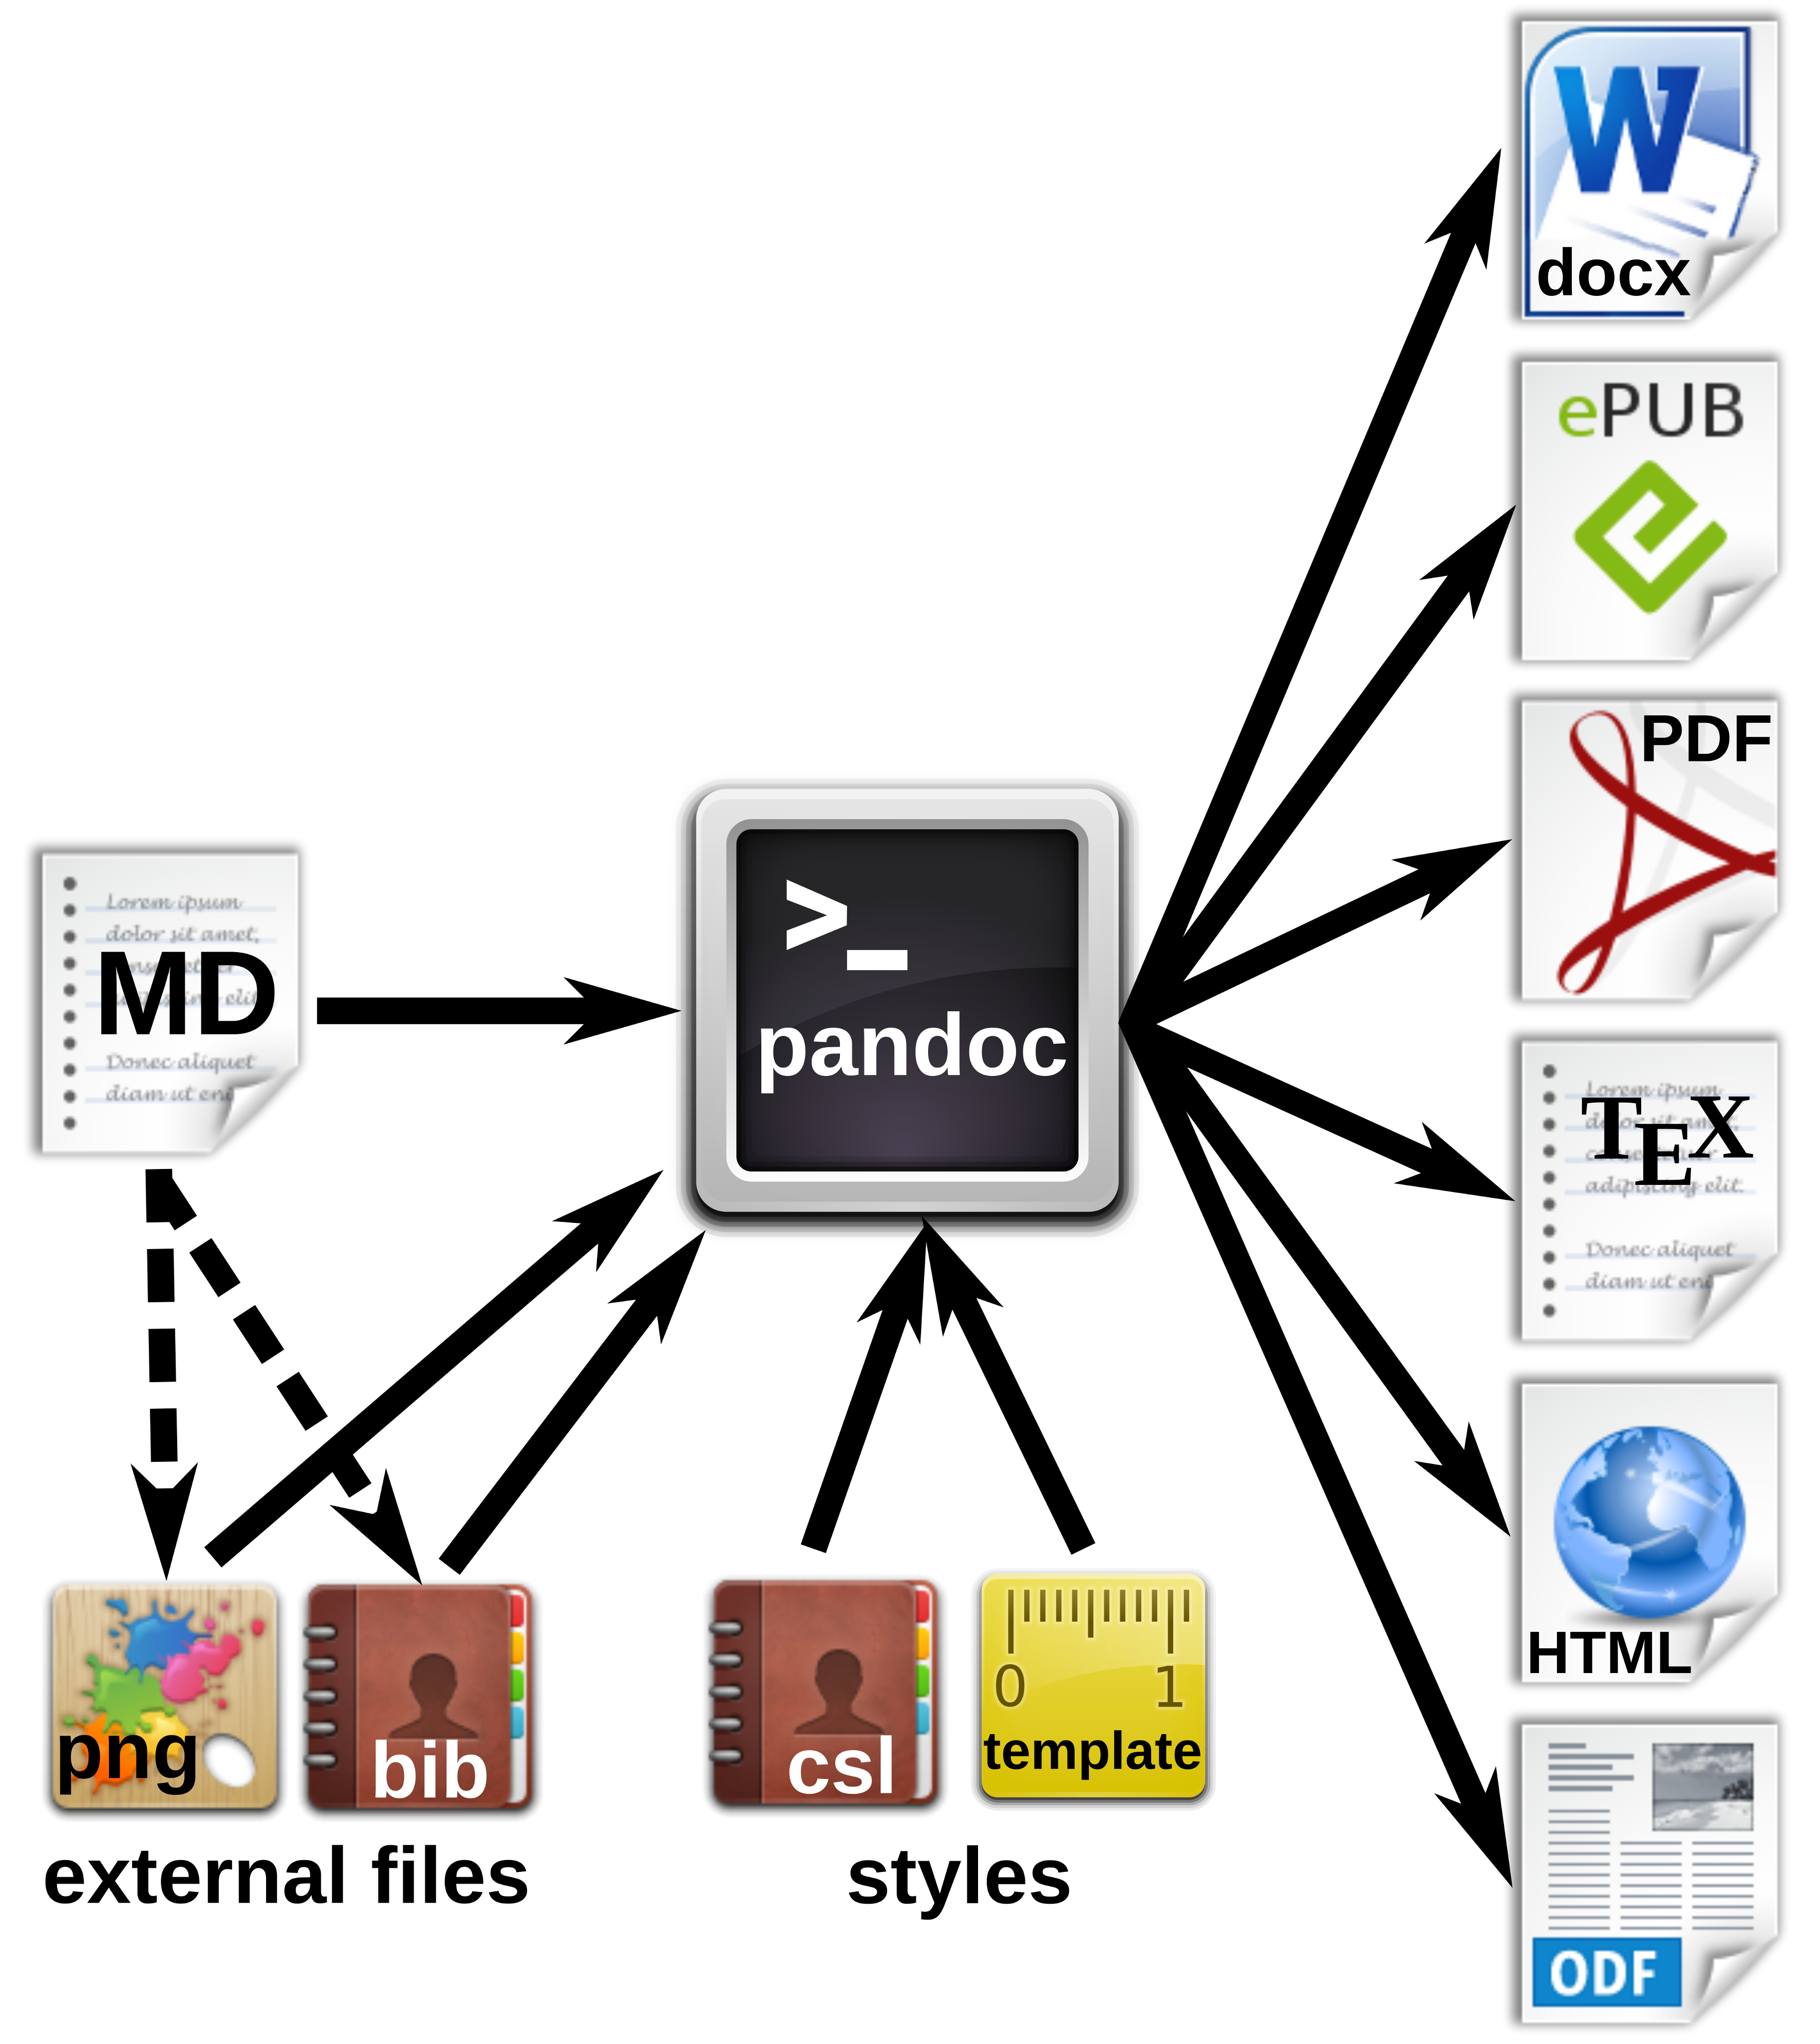
\includegraphics{fig-pandoc-workflow.png}
\textbf{Figure
3.}
Workfow
for
the
generation
of
multiple
document
formats
with
pandoc.

\section{Markdown
editors
and
online
editing}\label{markdown-editors-and-online-editing}

For
the
end
user,
the
convenience
of
work
with
text,
either
writing
alone
or
with
several
co-authors
is
important.
Therefore,
in
this
section
we
present
software
and
strategies
for
different
scenarios.
\textbf{Fig.
4}
summarized
various
options
for
local
or
networked
editing
of MD
files.

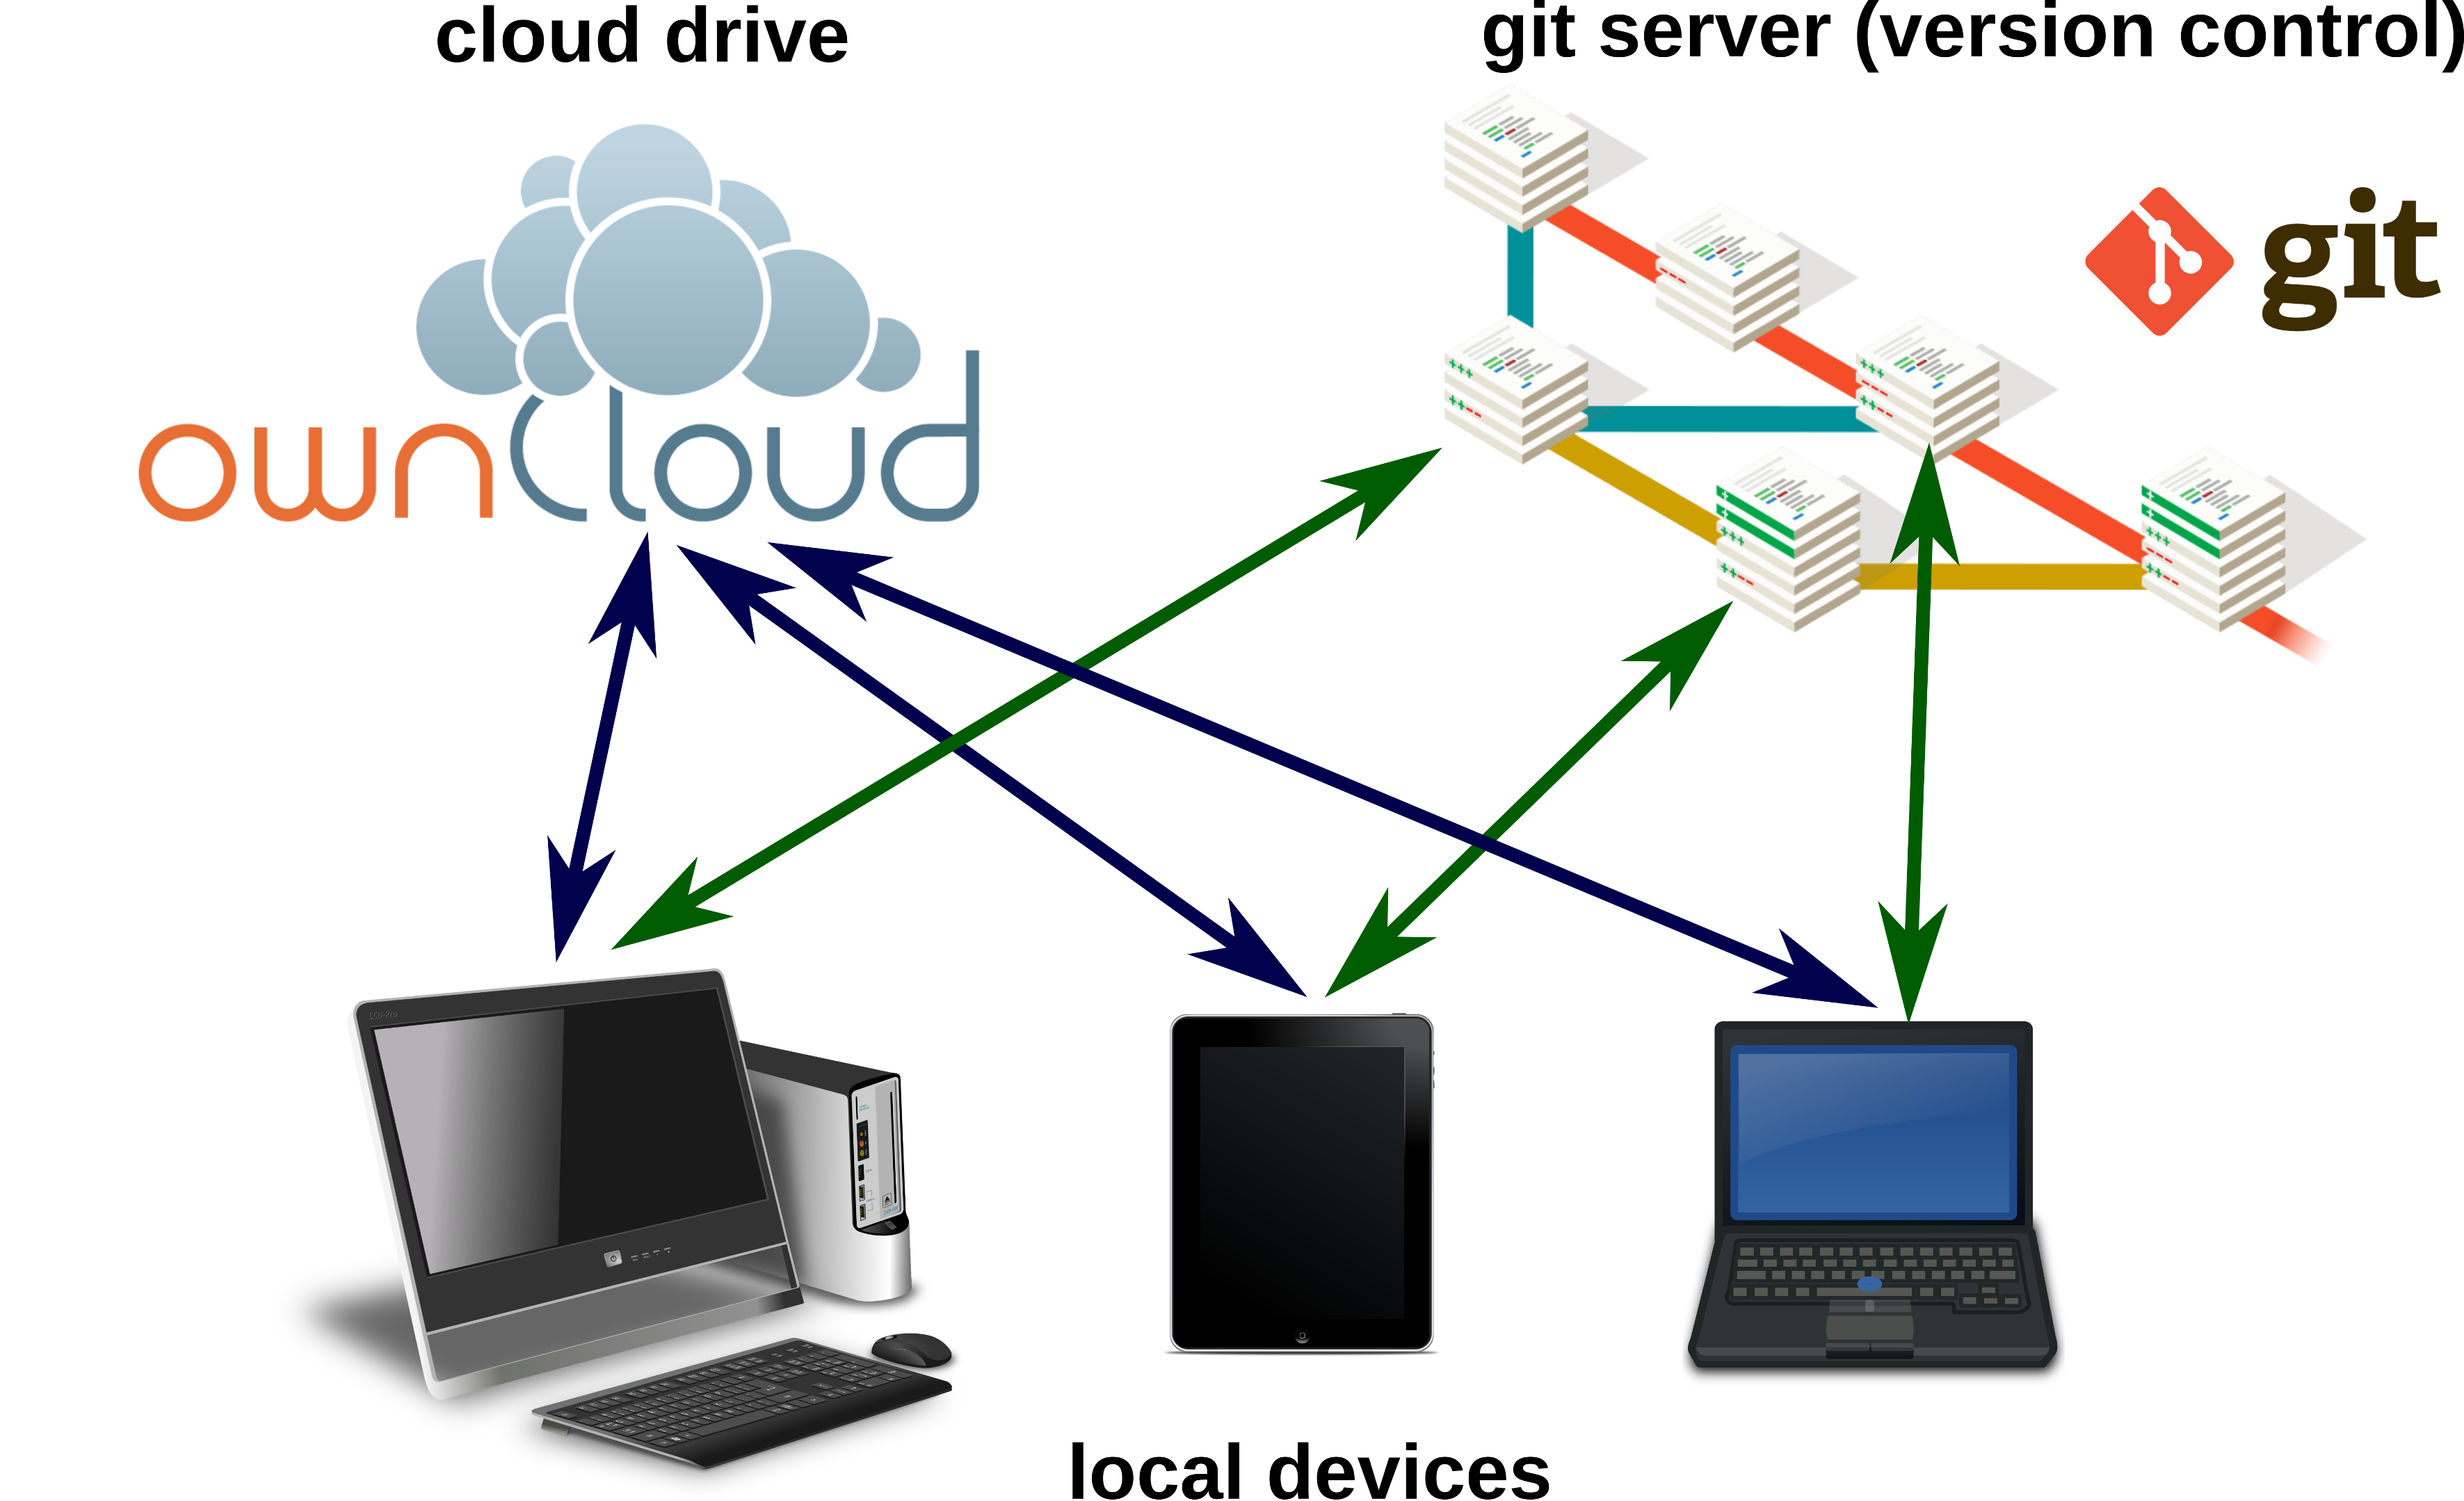
\includegraphics{fig-editing-options.png}

\textbf{Figure
4.}
Markdown
files
can
be
edited
on
local
devices
or on
cloud
drives.
A
local
or
remote
git
repository
enables
advanced
advanced
version
control.

\subsection{Markdown
editors}\label{markdown-editors}

Because
of
the
simple
MD
syntax,
basically
any
text
editor
is
suitable
for
editing
markdown
files.
The
formatting
tags
are
written
in
plain
text
and
easy
to
remember.
Therefore,
the
author
is
not
distracted
by
looking
around
for
layout
options
with
the
mouse.
For
several
popular
text
editors,
such
as
vim
(\url{http://www.vim.org/}),
GNU
Emacs
(\url{https://www.gnu.org/software/emacs/}),
atom
(\url{https://atom.io/})
or
geany
(\url{http://www.geany.org/}),
plugins
provide
additional
functionality
for
markdown
editing,
e.g.~syntax
highlighting,
command
helpers,
live
preview
or
structure
browsing.
Also
various
dedicated
mardown
editors
have
been
published.
Many
of
those
are
cross-platform
compatible,
such
as
Abricotine
(\url{http://abricotine.brrd.fr/}),
Ghostview
(\url{https://github.com/wereturtle/ghostwriter})
and
CuteMarkEd
(\url{https://cloose.github.io/CuteMarkEd/}).
The
lightweight
format
is
also
ideal
for
writing
on
mobile
devices.
Numerous
applications
are
available
on
the
App
stors
for
Android
and
iOS
systems.
The
programs
Swype
and
Dragon
(\url{http://www.nuance.com/})
facilitate
the
input
of
text
on
such
devices
by
guessing
words
from
gestures
and
speach
recognition
(dictation).
\textbf{Fig.
5.}
shows
the
editing
of a
text
with
the
markdown
editor
CuteMarkEd.

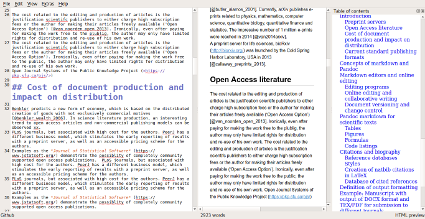
\includegraphics{fig-cutemarked-editor.png}
\textbf{Figure
5.}
Editing
window,
HTML
preview
and
table
of
contents
using
the
CuteMarkEd
editor.

\subsection{Online
editing
and
collaborative
writing}\label{online-editing-and-collaborative-writing}

Storing
manuscripts
on
network
drives
(\emph{The
Cloud})
has
become
popular
because
of
several
reasons:
Protection
against
data
loss,
synchronization
of
documents
between
several
devices
and
collaborative
editing
options.
Markdown
files
on a
Google
Drive
(\url{https://drive.google.com})
for
instance
can
be
edited
online
with
StackEdit
(\url{https://stackedit.io}).
m can
be
used
for
editing
markdown
files
.
\textbf{Fig.
6}
demonstrates
the
online
editing
of a
markdown
file
on an
OwnCloud
(\url{https://owncloud.com/})
installation,
using
a
plugin.

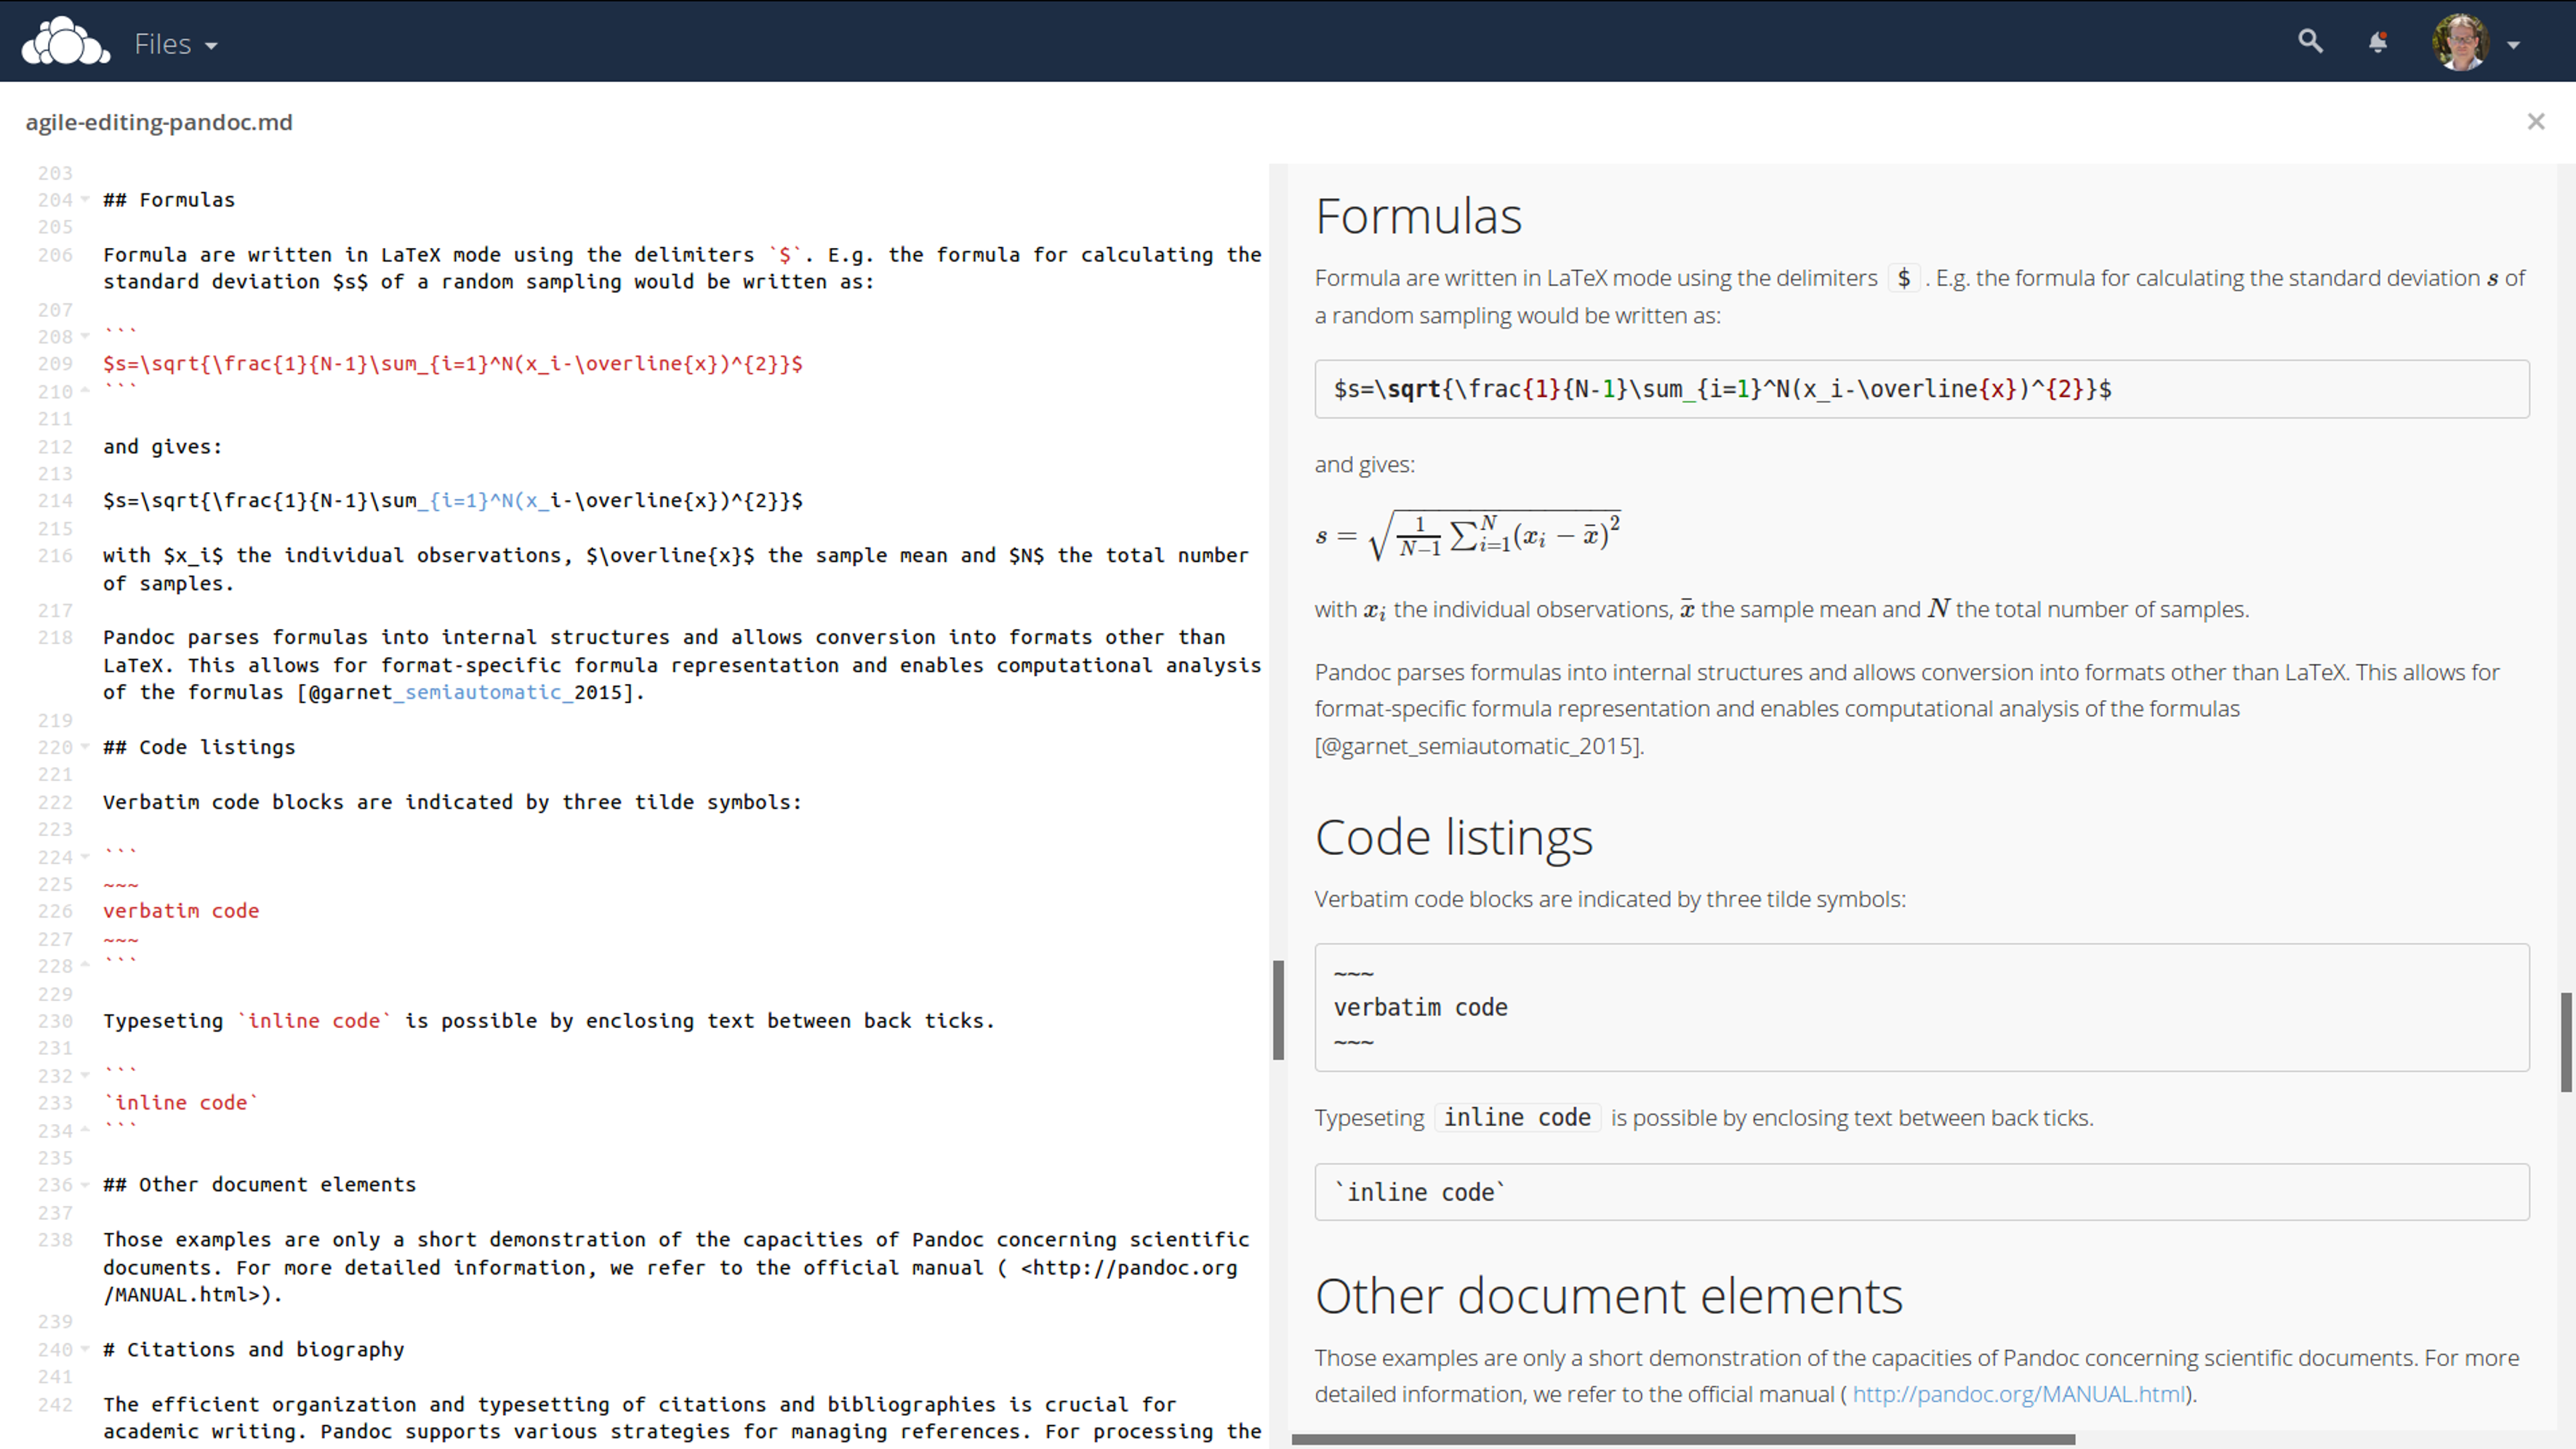
\includegraphics{fig-owncloud-md-editor.png}
\textbf{Figure
6.}
Direct
online
editing
of
this
manuscript
with
live
preview
using
the
ownCloud
Markdown
Editor
plugin
by
Robin
Appelman.

Even
formalas
are
rendered
correctly
in
the
HTML
live
preview
window
of
the
OwnCloud
markdown
plugin
(\textbf{Fig.
6} ).

\subsection{Document
versioning
and
change
control}\label{document-versioning-and-change-control}

Programmers,
especially
when
working
in
distributed
teams,
rely
on
version
control
systems
to
manage
changes
of
code.
Currently,
Git
(\url{https://git-scm.com/}),
which
is
also
used
e.g.~for
the
development
of
the
Linux
kernel,
is
one
of
the
most
employed
software
solutions
for
versioning.
Git
allows
the
parallel
work
of
collaborators
and
has
an
efficient
merging
and
conflict
resolution
system.
A Git
respository
may
be
used
from
a
single
local
author
to
keep
track
of
changes,
or by
a
team
with
a
remote
repository,
e.g.~on
github
(\url{https://github.com/})
or
bitbucket
(\url{https://bitbucket.org/}).

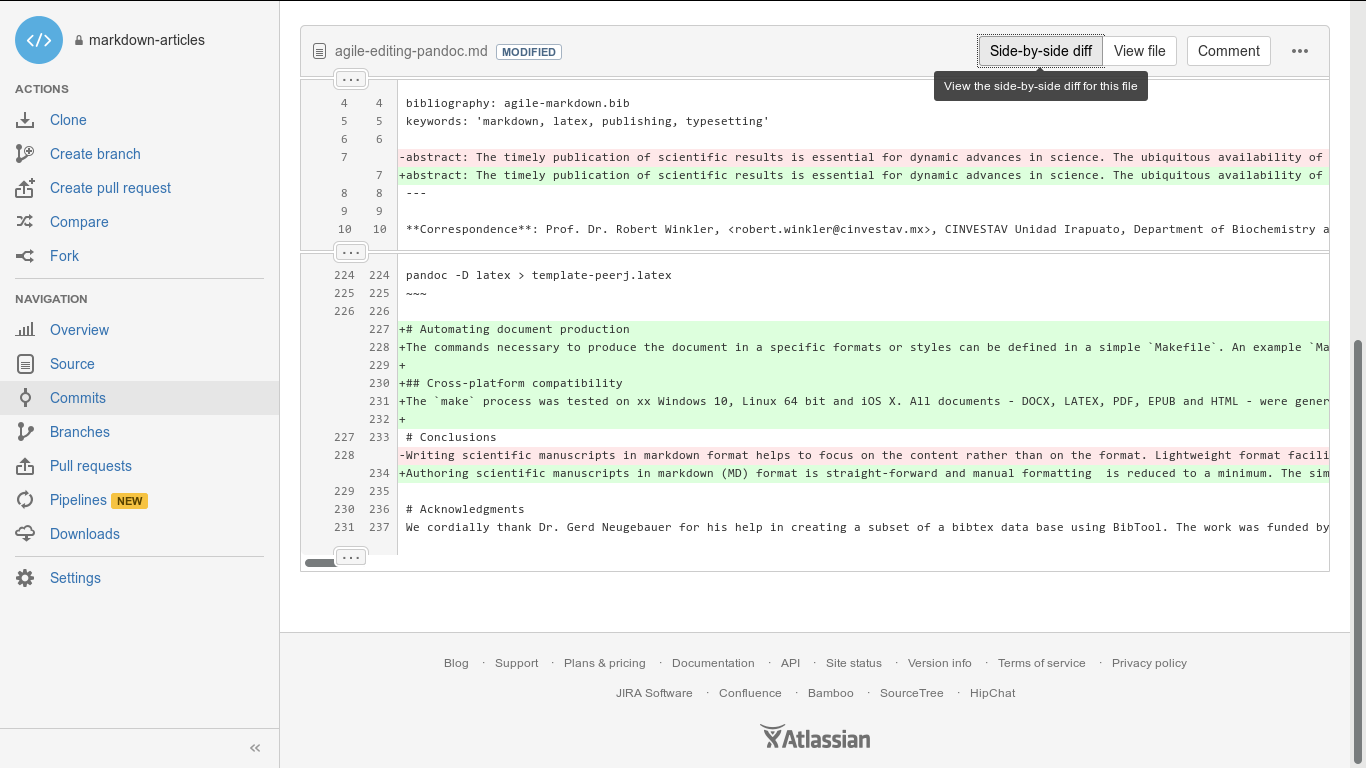
\includegraphics{fig-bitbucket-diff.png}
\textbf{Figure
7.}
Version
control
and
collaborative
editing
using
a git
repository
on
bitbucket.

For
the
writing
of
the
present
article,
the
co-authors
(Germany
and
Mexico)
used
a
remote
Git
repository
on
bitbucket.
The
plain
text
syntax
of
markdown
facilitates
the
visualization
of
differences
of
document
versions,
as
shown
in
\textbf{Fig.
7}.

\section{Pandoc
markdown
for
scientific
texts}\label{pandoc-markdown-for-scientific-texts}

Following,
the
potential
of
typesetting
scientific
manuscripts
with
pandoc
is
demonstrated
with
examples
for
typical
document
elements,
such
as
tables,
figures,
formulas,
code
listings
and
references.
A
brief
introduction
is
given
by
\citep{dominici_pandoc_2014}.
The
complete
Pandoc
User's
Manual
is
available
at
\url{http://pandoc.org/MANUAL.html}.

\subsection{Tables}\label{tables}

There
are
several
options
to
write
tables
in
markdown.
The
most
flexible
alternative
-
which
was
also
used
for
this
article
- are
pipe
tables.
The
contents
of
different
cells
are
separated
by
pipe
symbols
(\texttt{\textbar{}}):

\begin{verbatim}
Left | Center | Right | Default
:-----|:------:|------:|---------
 LLL  | CCC    | RRR   | DDD
\end{verbatim}

gives

\begin{longtable}[]{@{}lcrl@{}}
\toprule
\begin{minipage}[b]{0.17\columnwidth}\raggedright\strut
Left
\strut\end{minipage}
&
\begin{minipage}[b]{0.24\columnwidth}\centering\strut
Center
\strut\end{minipage}
&
\begin{minipage}[b]{0.20\columnwidth}\raggedleft\strut
Right
\strut\end{minipage}
&
\begin{minipage}[b]{0.27\columnwidth}\raggedright\strut
Default
\strut\end{minipage}\tabularnewline
\midrule
\endhead
\begin{minipage}[t]{0.17\columnwidth}\raggedright\strut
LLL
\strut\end{minipage}
&
\begin{minipage}[t]{0.24\columnwidth}\centering\strut
CCC
\strut\end{minipage}
&
\begin{minipage}[t]{0.20\columnwidth}\raggedleft\strut
RRR
\strut\end{minipage}
&
\begin{minipage}[t]{0.27\columnwidth}\raggedright\strut
DDD
\strut\end{minipage}\tabularnewline
\bottomrule
\end{longtable}

The
headings
and
the
alignment
of
the
cells
is
given
in
the
first
two
lines.
The
cell
width
is
variable.
The
pandoc
parameter
\texttt{-\/-columns=NUM}
can
be
used
to
define
the
length
of
lines
in
characters.
If
contents
do
not
fit,
they
will
be
wrapped.

\subsection{Figures}\label{figures}

Figures
are
inserted
as
follows:

\begin{verbatim}
![alt text](image location/ name)
\end{verbatim}

e.g.

\begin{verbatim}
![Publishing costs](fig-hybrid-publishing-costs.png)
\end{verbatim}

The
\texttt{alt\ text}
is
used
e.g.~in
HTML
output.
Additional
parameters
such
as
image
width
are
possible.

\subsection{Symbols}\label{symbols}

Scientific
texts
often
require
special
characters,
e.g.~Greek
letters,
mathematical
and
physical
symbols
etc.

The
UTF-8
standard,
developed
and
maintained
by
\emph{Unicode
Consortium},
enables
the
use
of
characters
across
languages
and
computer
platforms.
The
encoding
is
defined
as
RFC
document
3629
of
the
Network
Working
group
\citep{rfc3629}
and
as
ISO
standard
ISO/IEC
10646:2014
\citep{international_organization_for_standardization_iso/iec_2014}.
Specifications
of
Unicode
and
code
charts
are
provided
on
the
Unicode
homopage
(\url{http://www.unicode.org/}).

In
pandoc
mardown
documents,
Unicode
characters
such
as °,
α , ä
, Å
can
be
inserted
directly
and
passed
to
the
different
output
documents.
For
the
correct
processing
of
UTF-8
encoding
in
LATEX,
the
use
of
the
\texttt{-\/-latex-engine=xelatex}
option
is
necessary,
further
the
use
of an
appropiate
font.
The
Times-like
XITS
font
(\url{https://github.com/khaledhosny/xits-math})
for
high
quality
typesetting
of
scientific
texts
can
be
set
in
the
LATEX
template:

\begin{verbatim}
\usepackage{unicode-math}
\setmainfont
[    Extension = .otf,
   UprightFont = *-regular,
      BoldFont = *-bold,
    ItalicFont = *-italic,
BoldItalicFont = *-bolditalic,
]{xits}
\setmathfont
[    Extension = .otf,
      BoldFont = *bold,
]{xits-math}
\end{verbatim}

To
facilitate
the
input
of
specific
characters,
so-called
mnemonics
can
be
enabled
in
some
editors
(e.g.~in
atom
by
the
\texttt{character-table}
package).
For
example,
the
2-character
Mnemonics
`:u'
gives
`ü'
(diaeresis),
or
'D*'
the
greek
Δ.
The
possible
character
mnemonics
and
character
sets
are
listed
in
RFC
1345
\citep{rfc1345}.

\subsection{Formulas}\label{formulas}

Formula
are
written
in
LATEX
mode
using
the
delimiters
\texttt{\$}.
E.g.
the
formula
for
calculating
the
standard
deviation
\(s\)
of a
random
sampling
would
be
written
as:

\begin{verbatim}
$s=\sqrt{\frac{1}{N-1}\sum_{i=1}^N(x_i-\overline{x})^{2}}$
\end{verbatim}

and
gives:

\(s=\sqrt{\frac{1}{N-1}\sum_{i=1}^N(x_i-\overline{x})^{2}}\)

with
\(x_i\)
the
individual
observations,
\(\overline{x}\)
the
sample
mean
and
\(N\)
the
total
number
of
samples.

Pandoc
parses
formulas
into
internal
structures
and
allows
conversion
into
formats
other
than
LATEX.
This
allows
for
format-specific
formula
representation
and
enables
computational
analysis
of
the
formulas
\citep{garnet_semiautomatic_2015}.

\subsection{Code
listings}\label{code-listings}

Verbatim
code
blocks
are
indicated
by
three
tilde
symbols:

\begin{verbatim}
~~~
verbatim code
~~~
\end{verbatim}

Typeseting
\texttt{inline\ code}
is
possible
by
enclosing
text
between
back
ticks.

\begin{verbatim}
`inline code`
\end{verbatim}

\subsection{Other
document
elements}\label{other-document-elements}

Those
examples
are
only
a
short
demonstration
of
the
capacities
of
pandoc
concerning
scientific
documents.
For
more
detailed
information,
we
refer
to
the
official
manual
(
\url{http://pandoc.org/MANUAL.html}).

\section{Citations
and
biography}\label{citations-and-biography}

The
efficient
organization
and
typesetting
of
citations
and
bibliographies
is
crucial
for
academic
writing.
Pandoc
supports
various
strategies
for
managing
references.
For
processing
the
citations
and
the
creation
of
the
bibliography,
the
command
line
parameter
\texttt{-\/-filter\ pandoc-citeproc}
is
used,
with
variables
for
the
reference
database
and
the
bibliography
style.
The
bibliography
will
be
located
automatically
at
the
header
\texttt{\#\ References}
or
\texttt{\#\ Bibliography}.

\subsection{Reference
databases}\label{reference-databases}

Pandoc
is
able
to
process
all
mainstream
literature
database
formats,
such
as
RIS,
BIB,
etc.
However,
for
maintaining
compatibility
with
LATEX/
BIBTEX,
the
use
of
BIB
databases
is
recommended.
The
used
database
either
can
be
defined
in
the
YAML
metablock
of
the
MD
file
(see
below)
or it
can
be
passed
as
parameter
when
calling
pandoc.

\subsection{Inserting
citations}\label{inserting-citations}

For
inserting
a
reference,
the
database
key
is
given
within
square
brackets,
and
indicated
by an
`@'.
It is
also
possible
to
add
information,
such
as
page:

\begin{verbatim}
[@suber_open_2012; @benkler_wealth_2006, 57 ff.]
\end{verbatim}

gives
\citep[57
ff.]{suber_open_2012, benkler_wealth_2006}.

\subsection{Styles}\label{styles}

The
Citation
Style
Language
(CSL)
\url{http://citationstyles.org/}
is
used
for
the
citations
and
bibliographies.
This
file
format
is
supported
e.g.~by
the
reference
management
programs
Mendeley
\url{https://www.mendeley.com/},
Papers
\url{http://papersapp.com/}
and
Zotero
\url{https://www.zotero.org/}.
CSL
styles
for
particular
journals
can
be
found
from
the
Zotero
style
repository
\url{https://www.zotero.org/styles}.
The
bibliography
style,
which
pandoc
should
use
for
the
target
document
can
be
chosen
or in
the
YAML
block
of
the
markdown
document
or
can
be
passed
as an
command
line
option.
The
later
is
more
recommendable,
because
distinct
bibliography
style
may
be
used
for
different
documents.

\subsection{\texorpdfstring{Creation
of
LATEX
\texttt{natbib}
citations}{Creation of LATEX natbib citations}}\label{creation-of-latex-natbib-citations}

For
citations
in
scientific
manuscripts
written
in
LATEX,
the
natbib
package
is
widely
used.
To
create
a
LATEX
output
file
with
natbib
citations,
pandoc
simply
has
to be
run
with
the
\texttt{-\/-natbib}
option,
but
without
the
\texttt{-\/-filter\ pandoc-citeproc}
parameter.

\subsection{Database
of
cited
references}\label{database-of-cited-references}

To
share
the
bibliography
for a
certain
manuscript
with
co-authors
or
the
publisher's
production
team,
it is
often
desirable
to
generate
a
subset
of a
larger
database,
which
only
contains
cited
references.
If
LATEX
output
was
generated
with
the
\texttt{-\/-natbib},
the
compilation
of
the
file
with
LATEX
gives
an
AUX
file
(in
the
example
named
\texttt{md-article.aux}),
which
subsequently
can
be
extracted
using
BibTool
\url{https://github.com/ge-ne/bibtool}:

\begin{verbatim}
~~~
bibtool -x md-article.aux -o bibshort.bib
~~~
\end{verbatim}

In
this
example,
the
article
database
will
be
called
\texttt{bibshort.bib}.

For
the
direct
creation
of an
article
specific
BIB
database
without
using
LATEX,
we
wrote
a
simple
Perl
script
\texttt{mdbibexport}
(\url{https://github.com/robert-winkler/mdbibexport}).

\section{Meta
information
of
the
document}\label{meta-information-of-the-document}

Document
information
such
as
title,
authors,
abstract
etc.
can
be
defined
in a
metadata
block
written
in
YAML
syntax.
YAML
(``YAML
Ain't
Markup
Language'',
\url{http://yaml.org/})
is a
data
serialization
standard
with
simple,
human
readable
format.
Variables
defined
in
the
YAML
section
are
processed
by
pandoc
and
integrated
into
the
generated
documents.
The
YAML
metadata
block
is
recognized
by
three
hyphens
(\texttt{-\/-\/-})
at
the
beginning,
and
three
hyphens
or
dots
(\texttt{...})
at
the
end,
e.g.:

\begin{verbatim}
---
title: Formatting Open Science
author: 'Albert Krewinkel$^1$ and Robert Winkler$^{2,\star}$'
bibliography: agile-markdown.bib
---
\end{verbatim}

Using
the
LATEX
syntax
for
superscripts
(\texttt{\$\^{}\{2,*\}\$})
enables
the
correct
processing
for
different
output
formats.

\section{Example:
Manuscript
with
output
of
DOCX/
ODT
format
and
LATEX/
PDF
for
submission
to
different
journals.}\label{example-manuscript-with-output-of-docx-odt-format-and-latex-pdf-for-submission-to-different-journals.}

At
this
moment,
DOCX
the
most
common
format
for
manuscript
submission.
Some
publishers
also
ask
for
LATEX
or
accept
ODT.
In
this
example,
we
want
to
create
a
manuscript
for a
\emph{PLoS}
journal,
in
DOCX
and
ODT
for
WYSIWYG
word
processors.
Further,
a
version
in
LATEX/
PDF
should
be
produced
for
PeerJ
submission
and
archiving
at
the
PeerJ
preprint
server.

\subsection{Development
of
DOCX
template}\label{development-of-docx-template}

A
first
DOCX
document
with
bibliography
in
\emph{PLoS}
format
is
created
with
pandoc
DOCX
output:

\begin{verbatim}
pandoc -S -s --csl=plos.csl --filter pandoc-citeproc
-o pandoc-manuscript.docx agile-editing-pandoc.md
\end{verbatim}

The
document
settings
and
styles
of
the
resulting
file
\texttt{pandoc-manuscript.docx}
can
be
modified,
and
following
it
can
be
used
as
document
template
(\texttt{-\/-reference-docx=pandoc-manuscript.docx}).

\begin{verbatim}
pandoc -S -s --reference-docx=pandoc-manuscript.docx
--csl=apa.csl --filter pandoc-citeproc -o outfile.docx agile-editing-pandoc.md
\end{verbatim}

It is
also
possible
to
directly
re-use
a
previous
output
file
as
template
(i.e.~template
and
output
file
have
the
same
file
name):

\begin{verbatim}
pandoc -S -s --columns=10 --reference-docx= pandoc-manuscript.docx --csl=apa.csl --filter pandoc-citeproc -o pandoc-manuscript.docx agile-editing-pandoc.md
\end{verbatim}

In
this
way,
the
template
can
be
incrementally
adjusted
to
the
desired
document
formatting.
The
final
document
may
be
employed
later
as
pandoc
template
for
other
manuscripts
with
the
same
specifications.
In
this
case,
running
pandoc
the
first
time
with
the
template,
the
contents
of
the
new
manuscript
would
be
filled
into
the
provided
DOCX
template.
A
page
with
DOCX
manuscript
formatting
of
this
article
is
shown
in
\textbf{Fig.
8}.

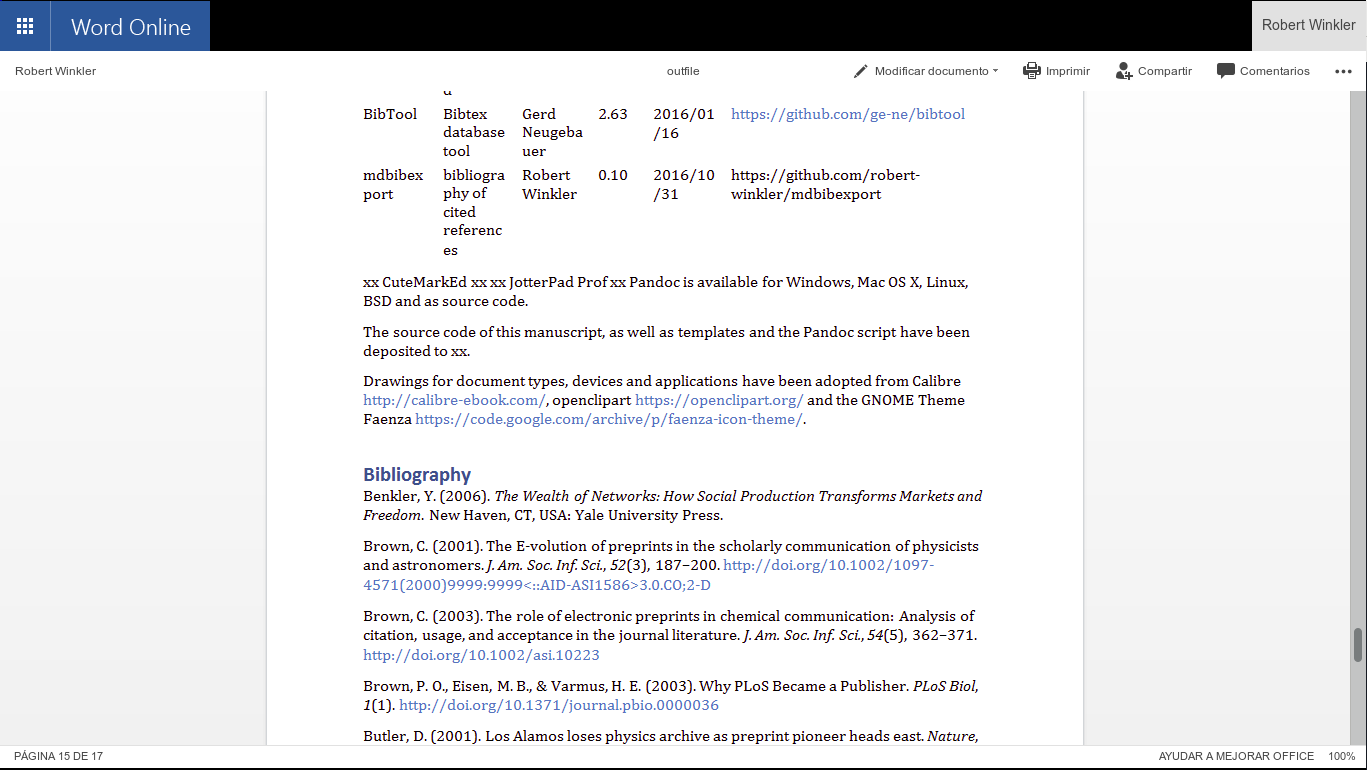
\includegraphics{fig-DOCX-document-in-O365.png}
\textbf{Figure
8.}
Editing
a
pandoc
generated
DOCX
in
Office
365.

The
same
proceedure
can
be
applied
for
an
ODT
formatted
document.

\subsection{Development
of a
TEX/PDF
template}\label{development-of-a-texpdf-template}

\begin{verbatim}
pandoc -D latex > template-peerj.latex
\end{verbatim}

\section{Automating
document
production}\label{automating-document-production}

The
commands
necessary
to
produce
the
document
in a
specific
formats
or
styles
can
be
defined
in a
simple
\texttt{Makefile}.
An
example
\texttt{Makefile}
is
included
in
the
source
code
of
this
preprint/
. The
desired
output
file
format
can
be
chosen
when
calling
\texttt{make}.
E.g.
\texttt{make\ outfile.pdf}
produces
this
preprint
in
PDF
format.Calling
\texttt{make}
without
any
option
creates
all
listed
document
types.

\subsection{Cross-platform
compatibility}\label{cross-platform-compatibility}

The
\texttt{make}
process
was
tested
on
Windows
10
and
Linux
64
bit.
All
documents
--
DOCX,
ODT,
LATEX,
PDF,
EPUB
and
HTML
--
were
generated
successfully,
which
demonstrates
the
cross-platform
compatibility
of
the
workflow.

\section{Conclusions}\label{conclusions}

Authoring
scientific
manuscripts
in
markdown
(MD)
format
is
straight-forward,
and
manual
formatting
is
reduced
to a
minimum.
The
simple
syntax
of MD
facilitates
the
document
editing
and
collaborative
writing.
The
rapid
conversion
of MD
to
multiple
formats
such
as
DOCX,
LATEX,
PDF,
EPUB
and
HTML
can
be
done
easily
using
pandoc,
and
templates
enable
the
automated
generation
of
documents
according
to
specific
journal
styles.
Altogether,
the
MD
format
supports
the
agile
writing
and
fast
production
of
scientific
literature.
The
associated
time
and
cost
reduction
especially
favours
community-driven
publication
strategies.

\section{Acknowledgments}\label{acknowledgments}

We
cordially
thank
Dr.~Gerd
Neugebauer
for
his
help
in
creating
a
subset
of a
bibtex
data
base
using
BibTool
and
Dr.~Ricardo
A.
Chávez
Montes
for
comments
on
the
manuscript.
The
work
was
funded
by
the
Consejo
Nacional
de
Ciencia
y
Tecnología
(CONACyT)
Mexico,
with
the
grant
FRONTERAS
2015-2/814
and
by
institutional
funding
of
the
Centro
de
Investigación
y de
Estudios
Avanzados
del
Instituto
Politécnico
Nacional
(CINVESTAV).

\section{Software
and
code
availability}\label{software-and-code-availability}

The
relevant
software
for
creating
this
manuscript
used
is
cited
according
to
\citep{smith_software_2016}
and
listed
in
\textbf{Tab.
3}.
Since
unique
identifiers
are
missing
for
most
software
projects,
we
only
refer
to
the
project
homepages
or
software
repositories:

\textbf{Table
3.}
Relevant
software
used
for
this
article.

\begin{longtable}[]{@{}llllll@{}}
\toprule
\begin{minipage}[b]{0.08\columnwidth}\raggedright\strut
\textbf{Software}
\strut\end{minipage}
&
\begin{minipage}[b]{0.20\columnwidth}\raggedright\strut
\textbf{Use}
\strut\end{minipage}
&
\begin{minipage}[b]{0.17\columnwidth}\raggedright\strut
\textbf{Authors}
\strut\end{minipage}
&
\begin{minipage}[b]{0.06\columnwidth}\raggedright\strut
\textbf{Version}
\strut\end{minipage}
&
\begin{minipage}[b]{0.06\columnwidth}\raggedright\strut
\textbf{Release}
\strut\end{minipage}
&
\begin{minipage}[b]{0.25\columnwidth}\raggedright\strut
\textbf{Homepage/
repository}
\strut\end{minipage}\tabularnewline
\midrule
\endhead
\begin{minipage}[t]{0.08\columnwidth}\raggedright\strut
pandoc
\strut\end{minipage}
&
\begin{minipage}[t]{0.20\columnwidth}\raggedright\strut
universal
markup
converter
\strut\end{minipage}
&
\begin{minipage}[t]{0.17\columnwidth}\raggedright\strut
John
MacFarlane
\strut\end{minipage}
&
\begin{minipage}[t]{0.06\columnwidth}\raggedright\strut
1.16.0.2
\strut\end{minipage}
&
\begin{minipage}[t]{0.06\columnwidth}\raggedright\strut
16/01/13
\strut\end{minipage}
&
\begin{minipage}[t]{0.25\columnwidth}\raggedright\strut
\url{http://www.pandoc.org}
\strut\end{minipage}\tabularnewline
\begin{minipage}[t]{0.08\columnwidth}\raggedright\strut
pandoc-citeproc
\strut\end{minipage}
&
\begin{minipage}[t]{0.20\columnwidth}\raggedright\strut
library
for
CSL
citations
with
pandoc
\strut\end{minipage}
&
\begin{minipage}[t]{0.17\columnwidth}\raggedright\strut
John
MacFarlane,
Andrea
Rossato
\strut\end{minipage}
&
\begin{minipage}[t]{0.06\columnwidth}\raggedright\strut
0.9.1
\strut\end{minipage}
&
\begin{minipage}[t]{0.06\columnwidth}\raggedright\strut
16/03/19
\strut\end{minipage}
&
\begin{minipage}[t]{0.25\columnwidth}\raggedright\strut
\url{https://github.com/jgm/pandoc-citeproc}
\strut\end{minipage}\tabularnewline
\begin{minipage}[t]{0.08\columnwidth}\raggedright\strut
ownCloud
\strut\end{minipage}
&
\begin{minipage}[t]{0.20\columnwidth}\raggedright\strut
personal
cloud
software
\strut\end{minipage}
&
\begin{minipage}[t]{0.17\columnwidth}\raggedright\strut
ownCloud
GmbH,
Community
\strut\end{minipage}
&
\begin{minipage}[t]{0.06\columnwidth}\raggedright\strut
9.1.1
\strut\end{minipage}
&
\begin{minipage}[t]{0.06\columnwidth}\raggedright\strut
16/09/20
\strut\end{minipage}
&
\begin{minipage}[t]{0.25\columnwidth}\raggedright\strut
\url{https://owncloud.org/}
\strut\end{minipage}\tabularnewline
\begin{minipage}[t]{0.08\columnwidth}\raggedright\strut
Markdown
Editor
\strut\end{minipage}
&
\begin{minipage}[t]{0.20\columnwidth}\raggedright\strut
plugin
for
ownCloud
\strut\end{minipage}
&
\begin{minipage}[t]{0.17\columnwidth}\raggedright\strut
Robin
Appelman
\strut\end{minipage}
&
\begin{minipage}[t]{0.06\columnwidth}\raggedright\strut
0.1
\strut\end{minipage}
&
\begin{minipage}[t]{0.06\columnwidth}\raggedright\strut
16/03/08
\strut\end{minipage}
&
\begin{minipage}[t]{0.25\columnwidth}\raggedright\strut
\url{https://github.com/icewind1991/files_markdown}
\strut\end{minipage}\tabularnewline
\begin{minipage}[t]{0.08\columnwidth}\raggedright\strut
BibTool
\strut\end{minipage}
&
\begin{minipage}[t]{0.20\columnwidth}\raggedright\strut
Bibtex
database
tool
\strut\end{minipage}
&
\begin{minipage}[t]{0.17\columnwidth}\raggedright\strut
Gerd
Neugebauer
\strut\end{minipage}
&
\begin{minipage}[t]{0.06\columnwidth}\raggedright\strut
2.63
\strut\end{minipage}
&
\begin{minipage}[t]{0.06\columnwidth}\raggedright\strut
16/01/16
\strut\end{minipage}
&
\begin{minipage}[t]{0.25\columnwidth}\raggedright\strut
\url{https://github.com/ge-ne/bibtool}
\strut\end{minipage}\tabularnewline
\bottomrule
\end{longtable}

The
source
code
of
this
manuscript,
as
well
as
templates
and
the
pandoc
Makefile
have
been
deposited
to
https://github.com/robert-winkler/scientific-articles-markdown/.

Drawings
for
document
types,
devices
and
applications
have
been
adopted
from
Calibre
\url{http://calibre-ebook.com/},
openclipart
\url{https://openclipart.org/}
and
the
GNOME
Theme
Faenza
\url{https://code.google.com/archive/p/faenza-icon-theme/}.

\bibliography{agile-markdown.bib}

\end{document}
